\chapter{Geodesics in Kerr spacetime}
\label{s:gek}
\index{geodesic!in Kerr spacetime}

\minitoc

\section{Introduction}

\section{Equations of geodesic motion}

\subsection{Introduction}

In all this chapter, we are concerned by the motion of a particle
$\mathscr{P}$ in Kerr spacetime $(\M,\w{g})$, assuming that $\mathscr{P}$
feels only gravity, as described by $\w{g}$ (freely falling particle).
The worldline $\Li$ of $\mathscr{P}$
is then necessarily a geodesic\footnote{The definition and basic properties of geodesics
are recalled in Appendix~\ref{s:geo}; see also Sec.~\ref{s:fra:geod_motion}.} of
$(\M,\w{g})$. It is a timelike geodesic if $\mathscr{P}$ is a massive particle
and a null geodesic if $\mathscr{P}$ is massless (e.g. a photon).

In a given coordinate system $(x^\alpha)$, the geodesic $\Li$ is described
by a system of the form\footnote{In Appendices~\ref{s:bas} and \ref{s:geo},
we use a different notation for the function $X^\alpha(\lambda)$ defining
$\Li$ and the coordinate $x^\alpha$ (cf. Secs.~\ref{s:bas:vectors} and
\ref{s:geo:geodesic_eq}). Following standard usage in the physics literature,
we shall not do this in this chapter.}
$x^\alpha = x^\alpha(\lambda)$, where $\lambda$ is an
affine parameter\footnote{See Sec.~\ref{s:geo:def} for the definition
of an affine parameter along a geodesic.} along $\Li$. We choose $\lambda$ to be the affine parameter
associated with $\mathscr{P}$'s 4-momentum $\w{p}$ [cf. Eq.~(\ref{e:fra:p_dxdl})]. We have
then $\D x^\alpha / \D\lambda = p^\alpha$.
The curve $\Li$ is a geodesic iff the functions $x^\alpha(\lambda)$ obey
the geodesic equation [Eq.~(\ref{e:geo:eq_geod}) in Appendix~\ref{s:geo}]:
\be \label{e:gek:eq_geod}
    \frac{\D^2 x^\alpha}{\D\lambda^2} + \Gamma^\alpha_{\ \, \mu \nu}
    \frac{\D x^\mu}{\D\lambda} \frac{\D x^\nu}{\D\lambda} = 0 ,
\ee
where the $\Gamma^\alpha_{\ \, \mu \nu}$'s are the Christoffel symbols\index{Christoffel symbols} of the metric $\w{g}$
with respect to the coordinates $(x^\alpha)$, as given by Eq.~(\ref{e:bas:Christoffel}).
Equation~(\ref{e:gek:eq_geod}) is actually a system of four coupled second-order
differential equations, that are non-linear. We are going to see that in
order to compute the geodesics of Kerr spacetime, it is not necessary to
solve this system, since, as in the Schwarzschild case studied in Chap.~\ref{s:ges}, we have
enough first integrals of Eq.~(\ref{e:gek:eq_geod}) to reduce
the problem to four first-order equations
of the type $\D x^\alpha/\D\lambda = F^\alpha(x^0, x^1, x^2, x^3)$.

Three integrals of motion are similar to those in the Schwarzschild case.
One is the particle's mass $\mu$ (Sec.~\ref{s:gek:mass_int_motion} below)
and the two other ones are
the conserved energy $E$ and the conserved angular momentum
$L$ (Sec.~\ref{s:gek:int_motion_sym}), which arise from the common symmetries
of Kerr and Schwarzschild spacetimes: stationarity (outside the ergosphere) and axisymmetry.
In the Schwarzschild case, the fourth integral of motion was provided by
spherical symmetry, which constrained all geodesics to be planar, so that
a suitable choice of
coordinates $(t,r,\th,\ph)$ makes a given geodesic confined to the
hyperplane $\th=\pi/2$, yielding the first integral $p^\th=0$ [Eq.~(\ref{e:ges:pth_zero})].
The Kerr spacetime with $a\not=0$ being not spherically symmetric, we loose
this property here. Fortunaly there exists another
integral of motion: the Carter constant; it arises from a remarkable property
of Kerr spacetime: the existence of a non-trivial Killing tensor (Sec.~\ref{s:gek:Carter_const}).
With the particle mass $\mu$, this makes a total of four integral of motions,
which renders the problem integrable (Sec.~\ref{s:gek:first_order_system}).


\subsection{Integrals of motion from spacetime symmetries} \label{s:gek:int_motion_sym}

As for Schwarzschild spacetime (cf. Sec.~\ref{s:ges:fiom}), we have the following
property.
\begin{greybox}
The Killing vectors $\w{\xi}$ and $\w{\eta}$ of Kerr spacetime,
associated respectively with
stationarity and axisymmetry [cf. Eq.~(\ref{e:ker:def_xi_eta})],
give birth to two conserved quantities
along the geodesic $\Li$:
\begin{subequations}
\label{e:gek:def_E_L}
\begin{align}
& \encadre{E := - \w{\xi}\cdot \w{p} = - \w{g}(\w{\xi},\w{p}) } \label{e:gek:def_E} \\
& \encadre{L := \w{\eta}\cdot \w{p} = \w{g}(\w{\eta},\w{p}) } , \label{e:gek:def_L}
\end{align}
\end{subequations}
where $\w{p}$ is the 4-momentum of particle $\mathscr{P}$ (cf. Sec.~\ref{s:fra:worldlines}).
For the same reasons as in Sec.~\ref{s:ges:fiom}, $E$ is called
the \defin{conserved energy}\index{conserved!energy}\index{energy!conserved --}
or \defin{energy at infinity}\index{energy!at infinity} of $\mathscr{P}$,
while $L$ is called $\mathscr{P}$'s \defin{conserved angular momentum}\index{conserved!angular momentum}\index{angular momentum!conserved --}
or \defin{angular momentum at infinity}\index{angular momentum!at infinity}
of $\mathscr{P}$.
\end{greybox}
\begin{remark}
Asymptotically, the scalar $L$ is only the
component along the rotation axis of $\mathscr{P}$'s angular momentum vector $\w{L}$
as measured by an inertial observer at rest with respect to the black hole.
For this reason, it is sometimes denoted by $L_z$, instead of merely $L$.
\end{remark}

In coordinates $(t,r,\th,\ph)$ adapted to the spacetime symmetries,
i.e. coordinates such that $\w{\xi} = \wpar_t$ and $\w{\eta}=\wpar_\ph$,
for instance Boyer-Lindquist coordinates (Sec.~\ref{s:ker:expr_BL}),
Kerr coordinates (Sec.~\ref{s:ker:Kerr_coord}) or 3+1 Kerr coordinates
(Sec.~\ref{s:ker:3p1_Kerr_coord}), one can rewrite
(\ref{e:gek:def_E_L})
in terms of the components $p_t = g_{t\mu} \, p^\mu$ and $p_\ph = g_{\ph\mu} \, p^\mu$
of the 1-form $\uu{p}$ associated to $\w{p}$ by metric duality:
\begin{subequations}
\label{e:gek:E_pt_L_pph}
\begin{align}
& E = - p_t \\
& L = p_\ph
\end{align}
\end{subequations}
Indeed, in such a coordinate system, $\xi^\mu =  \delta^\mu_{\ \, t}$
and $\eta^\mu = \delta^\mu_{\ \, \ph}$, so that $E = -g_{\mu\nu} \, \xi^\mu p^\nu = -g_{t\nu} \, p^\nu = -p_t$
and $L = g_{\mu\nu} \, \eta^\mu p^\nu = g_{\ph\nu} \, p^\nu = p_\ph$.

\begin{example}[Generators of the event and inner horizons] \label{x:gek:null_generator_hor}
Let us take for $\Li$ a null geodesic generator of the event horizon $\Hor$
(cf. Sec.~\ref{s:gek:null_gen_hor}). $\Li$ is then an outgoing principal null
geodesic and the 4-momentum vector $\w{p}$ is proportional to the null vector
$\wl \equalH \w{\chi} = \w{\xi} + \Omega_H \w{\eta}$ [Eq.~(\ref{e:ker:l_eqH_chi})
and (\ref{e:ker:def_chi})].
By definition of a
generator of a null hypersurface (cf. Sec.~\ref{s:def:null_geod_gen}),
$\w{p}$ is normal to $\Hor$. Since the Killing vector fields $\w{\xi}$ and $\w{\eta}$
are tangent to $\Hor$ (for $\Hor$ is globally preserved by the
spacetime symmetries), we get immediately from
the definitions (\ref{e:gek:def_E_L}) $E=0$ and $L=0$.
Similarly, if $\Li$ is a null geodesic generator of the
inner horizon $\Hor_{\rm in}$, $\Li$ is an outgoing principal null
geodesic, with $\w{p}$ proportional to
the null normal
$\wl \stackrel{\Hor_{\rm in}}{=} \w{\chi}_{\rm in} = \w{\xi} + \Omega_{\rm in} \w{\eta}$
[Eq.~(\ref{e:ker:chi_in_ell}) and (\ref{e:ker:def_chi_in})], so that we
have $E=0$ and $L=0$ as well. Hence we conclude:
\be \label{e:gek:generator_hor_E_L_zero}
    \Li \ \mbox{null geodesic generator of}\ \Hor\ \mbox{or}\ \Hor_{\rm in}
   \  \Longrightarrow\  E = 0 \quad\mbox{and}\quad L = 0 .
\ee
\end{example}

In what follows, we are going to use Boyer-Lindquist coordinates
$(x^\alpha)=(t,r,\th,\ph)$
as introduced in Sec.~\ref{s:ker:expr_BL}.
Given the components (\ref{e:ker:metric_BL}) of the metric tensor $\w{g}$
in these coordinates, evaluating $E$ and $L$
via $E = - g_{t\mu} \, p^\mu$ and $L = g_{\ph\mu} \, p^\mu$ yields
\be \label{e:gek:E_first_int}
    E = \left( 1 - \frac{2 m r}{\rho^2} \right)\,  p^t
        + \frac{2 a m r \sin^2\th}{\rho^2}\,  p^\ph  .
\ee
\be \label{e:gek:L_first_int}
    L = - \frac{2 a m r \sin^2\th}{\rho^2} \, p^t
        + \left( r^2 + a^2 + \frac{2 a^2 m r \sin^2\th}{\rho^2} \right)
    \sin^2\th \,  p^\ph ,
\ee
where $\rho^2 := r^2 + a^2 \cos^2\th$ [Eq.~(\ref{e:ker:def_rho2})].

Let us recall that the components $(p^\alpha)$ of the 4-momentum are
related to the equation $x^\alpha = x^\alpha(\lambda)$ of the geodesic $\Li$
in terms of the affine parameter $\lambda$ by $p^\alpha = \D x^\alpha / \D\lambda$
[cf. Eq.~(\ref{e:fra:p_dxdl})], i.e.
\be \label{e:gek:pa_der_xa}
    p^t = \derd{t}{\lambda},\quad
    p^r = \derd{r}{\lambda},\quad
    p^\th = \derd{\th}{\lambda},\quad
    p^\ph = \derd{\ph}{\lambda} .
\ee

\subsection{Mass as an integral of motion} \label{s:gek:mass_int_motion}

The mass $\mu$ of particle $\mathscr{P}$ is related to the scalar square of
the 4-momentum vector $\w{p}$ via Eq.~(\ref{e:fra:def_mass}):
\be \label{e:gek:mu_gpp}
    \mu^2 = - \w{g}(\w{p}, \w{p}) .
\ee
The fact that $\Li$ is a geodesic implies that $\mu$ is a constant along
$\Li$ (cf. Eq.~(\ref{e:geo:vv_const}) in Appendix~\ref{s:geo}). It therefore
provides a third integral of motion, after $E$ and $L$.

It is convenient to express (\ref{e:gek:mu_gpp}) in terms of the inverse metric
in order to let appear $p_t = -E$ and $p_\ph = L$:
\[
    \mu^2 = - g^{\mu\nu} p_\mu p_\nu .
\]

Given the components (\ref{e:ker:inv_met_BL}) of the inverse metric
in Boyer-Lindquist coordinates, we get
\bea
    \mu^2 & = & \frac{1}{\Delta}
    \left( r^2 + a^2 + \frac{2 a^2 m r \sin^2\th}{\rho^2} \right) E^2
    -\frac{4 a m r}{\rho^2 \Delta} E L
    - \frac{1}{\Delta}\left(1 - \frac{2 m r}{\rho^2} \right) \frac{L^2}{\sin^2\th}
    \nonumber \\
   &  & - \frac{\rho^2}{\Delta} \left( p^r \right) ^2
    - \rho^2 \left( p^\theta \right) ^2 ,   \label{e:gek:mu2_first_int}
\eea
where $\Delta := r^2 - 2 m r + a^2$ [Eq.~(\ref{e:ker:def_Delta})].
Note that we have expressed $p_r$ and $p_\th$ in terms of $p^r$ and $p^\th$
thanks to the relations $p_r = g_{r\mu} p^\mu$ and $p_\th = g_{\th\mu} p^\mu$,
which are very simple for the Boyer-Lindquist components (\ref{e:ker:metric_BL})
of $\w{g}$:
\be \label{e:gek:p_r_p_th_cov_con}
    p_r = \frac{\rho^2}{\Delta} \, p^r
    \qquad\mbox{and}\qquad
    p_\th = \rho^2 \, p^\th .
\ee

\subsection{The fourth integral of motion: Carter constant} \label{s:gek:Carter_const}

It turns out that the Kerr spacetime is endowed with a non-trivial
Killing tensor of valence 2: the
\defin{Walker-Penrose Killing tensor}\index{Killing!tensor!Walker-Penrose --}\index{Walker-Penrose Killing tensor} $\w{K}$, which is the symmetric tensor of type
$(0,2)$ defined by
\be \label{e:gek:def_K}
    \encadre{ \w{K} := (r^2 + a^2) \left( \uu{k} \otimes \uu{\el} + \uu{\el} \otimes \uu{k} \right) + r^2 \w{g} } ,
\ee
where $\uu{\el}$ and $\uu{k}$ are the 1-forms associated by metric duality
to the null vector fields $\w{k}$ and $\wl$ tangent to the principal null
geodesics introduced in Sec.~\ref{s:ker:principal_geod}. In index notation,
Eq.~(\ref{e:gek:def_K}) writes
\be
    K_{\alpha\beta} = (r^2 + a^2) \left(k_\alpha \el_\beta + \el_\alpha k_\beta \right)
        + r^2 g_{\alpha\beta} .
\ee
$\w{K}$ is called a \defin{Killing tensor}\index{Killing!tensor} because its symmetrized covariant derivative vanishes identically:
\be \label{e:gek:Killing_eq_K}
    \encadre{ \nabla_{(\alpha} K_{\beta\gamma)} = 0 }.
\ee
This property can be seen as a generalization of the Killing equation
(\ref{e:neh:Killing_equation}) to tensors of valence 2.
That the tensor $\w{K}$ defined by (\ref{e:gek:def_K}) obeys the Killing
identity (\ref{e:gek:Killing_eq_K}) is shown in the notebook~\ref{s:sam:Kerr_Killing_tensor}.

Killing tensors are discussed in Sec.~\ref{e:geo:Killing_tensor} of Appendix~\ref{s:geo}.
It is shown there that the Killing identity (\ref{e:gek:Killing_eq_K}) implies that
the following quantity is constant along any geodesic $\Li$ [cf. Eq.~(\ref{e:geo:Kvv_const})]:
\be
    \encadre{ \mathscr{K} := \w{K}(\w{p}, \w{p}) = K_{\mu\nu} p^\mu p^\nu } .
\ee
$\mathscr{K}$ is named \defin{Carter constant}\index{Carter!constant}.
From the definition (\ref{e:gek:def_K}) of $\w{K}$, we have
\be \label{e:gek:Kcarter_prov}
    \mathscr{K} = 2(r^2 + a^2) \langle \uu{k}, \w{p} \rangle
        \langle \uu{\el}, \w{p} \rangle + r^2 \w{g}(\w{p}, \w{p}).
\ee
Now by Eq.~(\ref{e:gek:mu_gpp}), $\w{g}(\w{p}, \w{p}) = - \mu^2$. Besides, we
have
\[
  \langle \uu{k}, \w{p} \rangle = k_\mu p^\mu = k^\mu p_\mu .
\]
The last form allows us to let appear the constants of motion $p_t = -E$ and
$p_\ph = L$ [Eq.~(\ref{e:gek:E_pt_L_pph})]. Using it with the components
of $\w{k}$ as given by Eq.~(\ref{e:ker:k_BL}), we get
\[
    \langle \uu{k}, \w{p} \rangle = - \frac{r^2 + a^2}{\Delta} E
    - p_r + \frac{a}{\Delta} L .
\]
Similarly, from the components (\ref{e:ker:ell_BL}) of $\wl$, we obtain
\[
     \langle \uu{\el}, \w{p} \rangle = - \frac{1}{2} E + \frac{\Delta}{2(r^2 + a^2)} p_r
     + \frac{a}{2(r^2 + a^2)} L .
\]
Accordingly, Eq.~(\ref{e:gek:Kcarter_prov}) becomes
\[
    \mathscr{K} = \frac{1}{\Delta} \left[ (r^2 + a^2) E + \Delta p_r - a L \right]
      \left[ (r^2 + a^2) E - \Delta p_r - a L \right] - r^2 \mu^2 ,
\]
which can be rewritten as
\be \label{e:gek:Kcarter_first_int}
   \encadre{ \mathscr{K} = \frac{1}{\Delta} \left[ \left( (r^2 + a^2) E - a L \right)^2
        - \rho^4 (p^r)^2 \right] - r^2 \mu^2 }.
\ee
Note that we have expressed $p_r$ in terms of $p^r$ via Eq.~(\ref{e:gek:p_r_p_th_cov_con}).

We can get some physical interpretation of the Carter constant from the above
expression, in the case where the particle $\mathscr{P}$ following the
geodesic $\Li$ visits the asymptotic region $r\to+\infty$. Indeed, given
that $\Delta := r^2 - 2m r + a^2 \sim r^2$  and $\rho^4 := (r^2 + a^2\cos^2\th)^2 \sim r^4$
as $r\to+\infty$, we deduce from Eq.~(\ref{e:gek:Kcarter_first_int})
that
\be \label{e:gek:Kcarter_r_inf}
    \mathscr{K} \underset{r\to + \infty}{\sim} r^2 \left[ E^2 - \mu^2 - (p^r)^2 \right] .
\ee
Then let $\Obs$ be the asymptotic inertial observer at rest with respect to the
black hole, i.e. the observer with $r\gg m$ and whose 4-velocity
coincides with the Killing vector
$\w{\xi} = \wpar_t$. $E$ is then $\mathscr{P}$'s energy as measured by $\Obs$
[cf. Eq.~(\ref{e:fra:E_obs}) and (\ref{e:gek:def_E})], so that, according to
Einstein's formula (\ref{e:fra:E2_m2_P2}), $E^2 - \mu^2 = \w{P}\cdot\w{P}$, where
$\w{P}$ is $\mathscr{P}$'s linear momentum as measured by $\Obs$. Given
that asymptotically, $p^r\sim P^r$ [cf. Eq.~(\ref{e:fra:p_E_P})],
Eq.~(\ref{e:gek:Kcarter_r_inf}) becomes
\[
    \mathscr{K} \underset{r\to + \infty}{\sim} r^2 \left[ \w{P}\cdot\w{P} - (P^r)^2 \right]
    = r^2 \left[ (P^{(\th)})^2 + (P^{(\ph)})^2 \right],
\]
where $P^{(\th)} = r P^\th \sim r p^\th$ and $P^{(\ph)} = r\sin\th\, P^\ph \sim r\sin\th\, p^\ph$
are the angular components of $\w{P}$ in the
orthonormal basis $(\w{e}_{(r)}, \w{e}_{(\th)}, \w{e}_{(\ph)}) := (\wpar_r, r^{-1} \wpar_\th,
(r\sin\th)^{-1}\wpar_\ph)$.
Now the total angular momentum of $\mathscr{P}$ measured by $\Obs$ is
\[
    \w{L}_{\rm tot} = \w{r} \times \w{P} = - r P^{(\ph)} \w{e}_{(\th)}
        + r P^{(\th)} \w{e}_{(\ph)} .
\]
Hence we may conclude that asymptotically, the Carter constant coincides with
the square of $\w{P}$'s angular momentum as measured by the inertial observer $\Obs$:
\be \label{e:gek:Kcarter_asymptot}
    \mathscr{K} \underset{r\to + \infty}{\sim} \w{L}_{\rm tot} \cdot \w{L}_{\rm tot} .
\ee

A useful result is
\begin{greybox}
A null geodesic $\Li$ has a vanishing Carter constant $\mathscr{K}$ if, and
only if, $\Li$ is a principal null geodesic:
\be \label{e:gek:K_zero_null}
   \mathscr{K} = 0 \iff \Li = \Li^{\rm in}_{(v,\th,\tph)} \quad\mbox{or}\quad
        \Li = \Li^{\rm out}_{(u,\th,\tilde{\tph})} ,
\ee
where $\Li^{\rm in}_{(v,\th,\tph)}$ (resp. $\Li^{\rm out}_{(u,\th,\tilde{\tph})}$)
stands for one of the ingoing (resp. outgoing) principal null geodesic
introduced in Sec.~\ref{s:ker:principal_geod}.
\end{greybox}
\begin{proof}
Consider expression (\ref{e:gek:Kcarter_prov}) for $\mathscr{K}$. If $\Li$
is a null geodesic, the term $\w{g}(\w{p},\w{p})$ vanishes identically, so that
one is left with
\[
    \mathscr{K} = 2 (r^2 + a^2) (\w{k}\cdot\w{p}) (\wl\cdot\w{p}) .
\]
Given that $r^2 + a^2\neq 0$ (this is clear for $a\neq 0$, while if $a=0$,
$r=0$ is excluded), we have then
\[
     \mathscr{K} = 0 \iff \w{k}\cdot\w{p} = 0 \quad\mbox{or}\quad \wl\cdot\w{p} = 0 .
\]
The vectors $\w{k}$, $\wl$ and $\w{p}$ are all null.
Now, according to the Corollary~2 in Sec.~\ref{s:fra:time_orientation},
two null vectors are orthogonal iff they are colinear. Hence
\[
    \mathscr{K} = 0 \iff \w{p} = \alpha \w{k} \quad\mbox{or}\quad \w{p} = \alpha \wl.
\]
Since $\w{k}$ (resp. $\wl$) is tangent to $\Li^{\rm in}_{(v,\th,\tph)}$ (resp.
$\Li^{\rm out}_{(u,\th,\tilde{\tph})}$), this completes the proof.
\end{proof}
Note that the result (\ref{e:gek:K_zero_null}) is consistent with the
interpretation (\ref{e:gek:Kcarter_asymptot}) of $\mathscr{K}$, since asymptotically
the principal null geodesics are purely radial\footnote{Indeed,
we deduce from Eqs.~(\ref{e:ker:k_BL}) and (\ref{e:ker:ell_BL}) that, for $r\to+\infty$,
$\w{k} \sim \wpar_t - \wpar_r$ and $\wl \sim (\wpar_t + \wpar_r)/2$.},
and hence have $\w{L}_{\rm tot} = 0$.

\begin{example}[Generators of the event and inner horizons]
We have seen in Example~\ref{x:gek:null_generator_hor} in Sec.~\ref{s:gek:int_motion_sym}
that the null geodesic generators of the event horizon $\Hor$ and the
inner horizon $\Hor_{\rm in}$ have $E=0$ and $L=0$.
Since these generators are principal null geodesics (cf.
Secs.~\ref{s:gek:null_gen_hor} and \ref{s:ker:Cauchy_hor}), the above results shows
that in addition $\mathscr{K}=0$. As $\mu=0$ by definition of a null geodesic,
we see that the four integrals of motion $\mu$, $E$, $L$ and $\mathscr{K}$ all
vanish for these geodesics.
\end{example}
The converse is true:
\begin{greybox}
The null geodesic generators of the event horizon $\Hor$ and of the
inner horizon $\Hor_{\rm in}$ are the only geodesics of Kerr spacetime
having their four integrals of motion vanishing:
\be \label{e:gek:all_const_zero}
\Li \ \mbox{null geodesic generator of}\ \Hor\ \mbox{or}\ \Hor_{\rm in} \iff
(\mu, E, L, \mathscr{K}) = (0, 0, 0, 0) .
\ee
\end{greybox}
\begin{proof}
If a geodesic $\Li$ has $(\mu,\mathscr{K}) = (0,0)$,
$\Li$ is necessary null and (\ref{e:gek:K_zero_null}) shows that
$\Li$ is a principal null geodesic. Moreover
Eq.~(\ref{e:gek:Kcarter_first_int}) with $(\mu, E, L, \mathscr{K}) = (0, 0, 0, 0)$
implies $p^r = 0$ (i.e. $\Li$ lies at a constant value of $r$).
If $\Li$ is ingoing, then $\w{p} \propto \w{k}$, with the Boyer-Lindquist components
of $\w{k}$ given by Eq.~(\ref{e:ker:k_BL}). Since $k^r = -1$, this precludes
$p^r = 0$. Hence $\Li$ is an outgoing principal null geodesic
and one has $\w{p} \propto \wl$, with the Boyer-Lindquist components
of $\wl$ given by Eq.~(\ref{e:ker:ell_BL}). We read $\ell^r = \Delta / (2(r^2+a^2))$
with $\Delta\neq 0$, except precisely on $\Hor$ and
$\Hor_{\rm in}$\footnote{This is graphically confirmed by
Figs.~\ref{f:ker:princ_null_geod_a90} and
\ref{f:ker:princ_null_geod_a50}, which show that $\Hor$ and $\Hor_{\rm in}$ are the only
locations where a principal null geodesic can have $r=\mathrm{const}$.}.
\end{proof}

\subsection{First order equations of motion} \label{s:gek:first_order_system}

We have thus obtained four first integrals of the geodesic equation
(\ref{e:gek:eq_geod}):
$E$ [Eq.~(\ref{e:gek:E_first_int})], $L$ [Eq.~(\ref{e:gek:L_first_int})],
$\mu^2$ [Eq.~(\ref{e:gek:mu2_first_int})] and $\mathscr{K}$
[Eq.~(\ref{e:gek:Kcarter_first_int})]. In the expressions of each of these integrals,
$p^\alpha$ has to be thought of as the first order derivative $\D x^\alpha/\D\lambda$
[Eq.~(\ref{e:gek:pa_der_xa})].
Two first integrals, namely $E$ and $L$, are linear in the $p^\alpha$'s, while
the two others, namely $\mu^2$ and $\mathscr{K}$, are quadratic.
Furthermore, Eqs.~(\ref{e:gek:E_first_int}) and (\ref{e:gek:L_first_int})
constitute a decoupled subsystem for $(p^t, p^\ph)$, which can easily be solved\footnote{An
intermediate step is combining  Eqs.~(\ref{e:gek:E_first_int}) and (\ref{e:gek:L_first_int})
to get $a E - L /\sin^2\th = a p^t - (r^2 + a^2) p^\ph$
and $(r^2 + a^2) E - a L = \Delta(p^t - a\sin^2\th p^\ph)$.},
yielding
\be \label{e:gek:rho2_pt}
    \rho^2 p^t = \frac{r^2 + a^2}{\Delta} [(r^2 + a^2) E - a L] + a ( L - a E \sin^2\th )
\ee
\be  \label{e:gek:rho2_pph}
    \rho^2 p^\ph = \frac{L}{\sin^2\th} - a E
    + \frac{a}{\Delta}\left[(r^2 + a^2) E - a L\right] .
\ee
Besides, Eq.~(\ref{e:gek:Kcarter_first_int}) involves only $p^r$ and can
be recast as
\be \label{e:gek:p_r_R}
    \rho^2 p^r = \eps_r \sqrt{ R(r) } ,
\ee
where $\eps_r := \operatorname{sgn} p^r = \pm 1$ and
$R(r)$ is the following 4th order polynomial of $r$:
\be \label{e:gek:def_R}
   \encadre{ R(r) := \left[ (r^2 + a^2) E - a L \right]^ 2 - \Delta (r^2 \mu^2 + \mathscr{K}) }.
\ee
In the above expression, let us recall that $\Delta$ is the function of $r$
given by Eq.~(\ref{e:ker:def_Delta}): $\Delta := r^2 - 2 m r + a^2$. All other
quantities are constant. Since $R(r)$ appeared first by rewriting Eq.~(\ref{e:gek:Kcarter_first_int}) as $\rho^4 (p^r)^2 = R(r)$, it has to fulfill
\be \label{e:gek:R_non_neg}
    \encadre{R(r) \geq 0 } .
\ee
In particular, this makes Eq.~(\ref{e:gek:p_r_R}) well posed.

Finally, if we substitute $p^r$ by the value given by Eqs.~(\ref{e:gek:p_r_R})-(\ref{e:gek:def_R}) in the mass first integral (\ref{e:gek:mu2_first_int}), we get, after simplification,
\be \label{e:gek:p_th_Th}
    \rho^2 p^\th = \eps_\th \sqrt{\Theta(\th)} ,
\ee
where $\eps_\th := \operatorname{sgn} p^\th = \pm 1$ and
\be \label{e:gek:def_Theta}
   \encadre{ \Theta(\th) := \mathscr{K} - \left(\frac{L}{\sin\th} - a E \sin\th \right)^2
        - \mu^2 a^2 \cos^2\th } .
\ee
Equation.~(\ref{e:gek:p_th_Th}) is actually derived from $\rho^4 (p^\th)^2 = \Theta(\th)$,
which imposes
\be \label{e:gek:Theta_non_neg}
    \encadre{\Theta(\th) \geq 0 } .
\ee

The following constant is often used instead of $\mathscr{K}$:
\be \label{e:gek:def_Q}
    \encadre{Q := \mathscr{K} - (L - a E)^2 }
\ee
Thanks to it, we may rewrite (\ref{e:gek:def_Theta}) as
\be \label{e:gek:Theta_Q}
    \encadre{ \Theta(\th) = Q + \cos^2\th \left[ a^2 (E^2 - \mu^2)
    - \frac{L^2}{\sin^2\th} \right] } .
\ee
Following the standard usage, we call $Q$ the \defin{Carter constant}\index{Carter!constant}
as well. To distinguish between the two Carter constants, we shall specify \emph{Carter constant $Q$}
or \emph{Carter constant $\mathscr{K}$}. As we shall see in Sec.~\ref{s:gek:th_motion},
$Q$ is well adapted to the description of the $\th$-motion of geodesics. On the other
hand, a nice property of $\mathscr{K}$, which is not shared by $Q$, is to be always non-negative,
as Eqs.~(\ref{e:gek:def_Theta}) and (\ref{e:gek:Theta_non_neg}) show:
\be
  \encadre{  \mathscr{K} \geq 0 }.
\ee

If the particle $\mathscr{P}$ reaches the asymptotic region $r\gg m$, we deduce from
Eqs.~(\ref{e:gek:def_Q}) and (\ref{e:gek:Kcarter_asymptot}) the following approximate
value of $Q$:
\be \label{e:gek:Q_Ltot2_L2}
   Q \underset{r\to + \infty}{\sim} \w{L}_{\rm tot} \cdot \w{L}_{\rm tot}
    - L^2 + a (2 L - a E^2) .
\ee
Hence, if $a=0$, $Q$ can be interpreted as the square of
the part of $\mathscr{P}$'s angular momentum (measured by the asymptotic inertial
observer) that is not in $L$.

\begin{remark}
One may derive the Carter constant $Q$ from a Killing tensor.
Indeed, from the Walker-Penrose Killing tensor $\w{K}$, let us form
the tensor field
\be \label{e:gek:def_tilde_K}
    \w{\tilde{K}} := \w{K} - \uu{\tilde{\eta}}\otimes\uu{\tilde{\eta}} ,
\ee
where
\be
    \w{\tilde{\eta}} := \w{\eta} + a \w{\xi} .
\ee
Being a linear combination with constant coefficients of the Killing vectors
$\w{\eta}$ and $\w{\xi}$, $\w{\tilde{\eta}}$ is itself a Killing vector.
It follows that $\uu{\tilde{\eta}}\otimes\uu{\tilde{\eta}}$ is a Killing tensor
(cf. Example~\ref{x:geo:trivial_Killing_tensors} in Sec.~\ref{e:geo:Killing_tensor}),
so that $\w{\tilde{K}}$ a Killing tensor. Applying it to the
4-momentum $\w{p}$, we get
\[
    \w{\tilde{K}}(\w{p},\w{p}) =  \underbrace{\w{K}(\w{p},\w{p})}_{\mathscr{K}}
        - (\underbrace{\langle\uu{\eta},\w{p}\rangle}_{L}
        + a \underbrace{\langle\uu{\xi},\w{p}\rangle}_{-E})^2 .
\]
Comparing with the definition (\ref{e:gek:def_Q}), we conclude that
\be
    Q = \w{\tilde{K}}(\w{p},\w{p}) .
\ee
As a side remark, we note that
the Boyer-Lindquist components of the contravariant tensor associated to $\w{\tilde{K}}$ by
metric duality have an expression particularly simple in terms of those of
the inverse metric (cf. the notebook~\ref{s:sam:Kerr_Killing_tensor}):
\be
    \tilde{K}^{\alpha\beta} = - a^2 \cos^2 \theta \, g^{\alpha\beta}
    + \operatorname{diag}(-a^2\cos^2\theta, 0, 1, \tan^{-2}\theta)^{\alpha\beta} .
\ee
\end{remark}

In view of the relation (\ref{e:gek:pa_der_xa}) between the $p^\alpha$'s
and the derivatives of the functions $x^\alpha(\lambda)$, we may
collect Eqs.~(\ref{e:gek:rho2_pt}), (\ref{e:gek:rho2_pph}), (\ref{e:gek:p_r_R})
and (\ref{e:gek:def_Theta}) as the first-order system
\begin{subequations}
\label{e:gek:eom_first_order}
\begin{align}
& \encadre{ \rho^2 \derd{t}{\lambda} = \frac{r^2 + a^2}{\Delta} [(r^2 + a^2) E - a L] + a ( L - a E \sin^2\th ) } \label{e:gek:dtdl} \\
& \encadre{ \rho^2 \derd{r}{\lambda} = \eps_r \sqrt{ R(r) } } \label{e:gek:drdl}\\
& \encadre{ \rho^2 \derd{\th}{\lambda} = \eps_\th \sqrt{\Theta(\th)} } \label{e:gek:dthdl}\\
& \encadre{ \rho^2 \derd{\ph}{\lambda}  = \frac{L}{\sin^2\th} - a E
    + \frac{a}{\Delta}\left[(r^2 + a^2) E - a L\right] } . \label{e:gek:dphdl}
\end{align}
\end{subequations}
The functions $R(r)$ and $\Theta(\th)$ are defined by Eq.~(\ref{e:gek:def_R})
and Eq.~(\ref{e:gek:def_Theta}) or (\ref{e:gek:Theta_Q}). They must obey
$R(r) \geq 0$ [Eq.~(\ref{e:gek:R_non_neg})] and $\Theta(\th) \geq 0$
[Eq.~(\ref{e:gek:Theta_non_neg})].
Note that besides the constants of motion $E$, $L$, $\mu$ and $\mathscr{K}$
or $Q$, $R(r)$ depends on $a$ and $m$ (via $\Delta$), while $\Theta(\th)$
depends on $a$ only.

In the system (\ref{e:gek:eom_first_order}), $\eps_r$
is $+1$ (resp. $-1$) in the parts of the geodesic $\Li$ where $r$ increases
(resp. decreases) with $\lambda$. Similarly, $\eps_\th$
is $+1$ (resp. $-1$) in the parts of $\Li$ where $\th$ increases
(resp. decreases) with $\lambda$.

\subsection{Turning points} \label{s:gek:turning_points}

Let $\Li$ be a geodesic that is not sticked at a constant value of the
coordinate $r$.
We define a \defin{$r$-turning point}\index{turning point!$r$-turning point} of $\Li$ as a point $p_0\in\Li$, the $r$-coordinate $r_0$ of which obeys
\be \label{e:gek:def_r_turning}
    R(r_0) = 0 \quad\mbox{and}\quad R'(r_0) \neq 0 ,
\ee
i.e. $r_0$ is a simple root of the polynomial $R$.

We have then
\be \label{e:gek:der_r_turning}
   \left. \derd{r}{\lambda} \right| _{\lambda_0} = 0
   \quad\mbox{and}\quad
   \left. \frac{\D^2 r}{\D\lambda^2} \right| _{\lambda_0} = \frac{R'(r_0)}{2\rho_0^4} \neq 0 ,
\ee
where $\lambda_0$ is the value of the affine parameter $\lambda$ at $p_0$
and $\rho_0 := \rho(p_0)$.
\begin{proof}
The vanishing of $\D r/\D\lambda$ at $\lambda_0$ follows immediately
from Eq.~(\ref{e:gek:drdl}) with $R(r_0)=0$, since $\rho^2$ never vanishes
on $\M$. Besides, by
taking the derivative of Eq.~(\ref{e:gek:drdl}) with respect to $\lambda$, we
get
\[
    2 \left(r \derd{r}{\lambda} + a^2 \cos\th\sin\th \derd{\th}{\lambda} \right)
    \derd{r}{\lambda} + \rho^2 \frac{\D^2 r}{\D\lambda^2} =
    \eps_r \frac{R'(r)}{2\sqrt{R(r)}} \derd{r}{\lambda} = \frac{R'(r)}{2\rho^2} .
\]
At $\lambda=\lambda_0$, the first term in left-hand side vanishes identically,
due to the $\D r/\D\lambda$ factor,
and we get the second part of (\ref{e:gek:der_r_turning}).
\end{proof}

We deduce from the result (\ref{e:gek:der_r_turning}) that at $\lambda=\lambda_0$,
$\D r/\D\lambda$ moves from positive to negative values or vice-versa
(depending on the sign of $R'(r_0)$), which means that the function $r(\lambda)$
switches from increasing to decreasing or vice-versa, hence the name
\emph{$r$-turning point}. The factor $\eps_r=\pm 1$ in Eq.~(\ref{e:gek:drdl}) necessarily
changes sign at $\lambda=\lambda_0$.

\begin{remark} \label{r:gek:der_r_analytic}
For a generic analytic function $r(\lambda)$ with $\D r/\D \lambda=0$ at
$\lambda_0$, the condition $\D^2 r/\D\lambda^2\neq 0$ at $\lambda_0$
is sufficient but not necessary for having $r$ change its direction of variation there.
Indeed, one can have the same property with $\D^2 r/\D\lambda^2= 0$ and higher order derivatives vanishing up to some even order $k$ for which
$\D^k r/\D\lambda^k\neq 0$. However, in the present case,
$\D^2 r/\D\lambda^2=0$ would imply $R'(r_0)=0$ and we shall see
Sec.~\ref{s:gek:asymptotic_values} that a geodesic can reach such a point only asymptotically,
i.e. for $\lambda\to +\infty$. Hence it cannot be a turning point.
\end{remark}


Similarly, if $\Li$ is a geodesic that is not sticked at a constant value of the
coordinate $\th$, we define a \defin{$\th$-turning point}\index{turning point!$\th$-turning point} of $\Li$ as a point $p_0\in\Li$, the
$\th$-coordinate $\th_0$ of which obeys
\be \label{e:gek:def_th_turning}
    \Theta(\th_0) = 0 \quad\mbox{and}\quad \Theta'(\theta_0) \neq 0 .
\ee
We deduce then from the equation of motion (\ref{e:gek:dthdl}):
\be \label{e:gek:der_th_turning}
   \left. \derd{\th}{\lambda} \right| _{\lambda_0} = 0
   \quad\mbox{and}\quad
   \left. \frac{\D^2 \th}{\D\lambda^2} \right| _{\lambda_0} = \frac{\Theta'(\th_0)}{2\rho_0^4} \neq 0 .
\ee
This implies that at a $\th$-turning point, the function $\th(\lambda)$
switches from increasing to decreasing or vice-versa. The factor $\eps_\th=\pm 1$ in Eq.~(\ref{e:gek:dthdl}) necessarily
changes sign at such a point.

\begin{remark}
A comment similar to Remark~\ref{r:gek:der_r_analytic} can be made:
a geodesic with varying $\th$ that has $\D\th/\D\lambda = 0$ for some finite
value of $\lambda$
cannot have $\D^2\th/\D\lambda^2 = 0$ at the same point, since we shall see
in Sec.~\ref{s:gek:asymptotic_values}
that a value of $\th$ with both $\Theta(\th)=0$
and $\Theta'(\th)=0$ can only be reached asymptotically along a geodesic.
Hence (\ref{e:gek:def_th_turning})
is a necessary and sufficient condition for a $\th$-turning point.
\end{remark}


\subsection{Equations of motion in terms of Mino time} \label{s:gek:Mino_time}

In view of the right-hand sides of the system (\ref{e:gek:eom_first_order}),
it is quite natural to introduce along the geodesic $\Li$ the new
parameter $\lambda'$ defined by
\be \label{e:gek:def_Mino_time}
    \D\lambda' = \frac{\D\lambda}{\rho^2}
     = \frac{\D\lambda}{r(\lambda)^2 + a^2 \cos^2 \th(\lambda)} .
\ee
Since $\rho^2$ never vanishes on the spacetime manifold $\M$ (by construction
of the latter, cf. Eq.~(\ref{e:ker:def_M_Kerr_spacetime})), the above relation
leads to a well-defined parameter along $\Li$. Moreover, since $\rho^2>0$, this
parameter increases towards the future, as $\lambda$. A difference between
the two parametrizations is that $\lambda'$ is not in general\footnote{The only
exception is for a circurlar orbit at $\theta=\pi/2$, since then $\rho^2$
is constant and Eq.~(\ref{e:gek:def_Mino_time}) defines an affine relation
between $\lambda$ and $\lambda'$.} an affine parameter
of $\Li$, contrary to $\lambda$.
The parameter $\lambda'$ is called \defin{Mino time}\index{Mino!time}\index{time!Mino --}
\cite{Mino03}.

In terms of Mino time, the system (\ref{e:gek:eom_first_order}) becomes
\begin{subequations}
\label{e:gek:eom_Mino}
\begin{align}
& \encadre{ \derd{t}{\lambda'} = \frac{r^2 + a^2}{\Delta} [(r^2 + a^2) E - a L] + a ( L - a E \sin^2\th ) } \label{e:gek:dtdl_Mino} \\
& \encadre{ \derd{r}{\lambda'} = \eps_r \sqrt{ R(r) } } \label{e:gek:drdl_Mino}\\
& \encadre{ \derd{\th}{\lambda'} = \eps_\th \sqrt{\Theta(\th)} } \label{e:gek:dthdl_Mino}\\
& \encadre{ \derd{\ph}{\lambda'}  = \frac{L}{\sin^2\th} - a E
    + \frac{a}{\Delta}\left[(r^2 + a^2) E - a L\right] } . \label{e:gek:dphdl_Mino}
\end{align}
\end{subequations}
It is remarkable that Eqs.~(\ref{e:gek:drdl_Mino}) and (\ref{e:gek:dthdl_Mino})
are two fully decoupled equations: Eq.~(\ref{e:gek:drdl_Mino}) is an ordinary
differential equation for the function $r(\lambda')$, while Eq.~(\ref{e:gek:dthdl_Mino})
is an ordinary differential equation for the function $\th(\lambda')$. This was
not the case for Eqs.~(\ref{e:gek:drdl}) and (\ref{e:gek:dthdl}) since $\rho^2$ is
a function of both $r$ and $\th$.

Equation~(\ref{e:gek:drdl_Mino}) can be integrated by the method of separation
of variables. On a part of $\Li$ where $R(r)\neq 0$, this yields
\be \label{e:gek:lp_int_dr_ov_R}
    \lambda' - \lambda'_0 =  \int_{r_0}^r \frac{\eps_r\, \D \bar{r}}{\sqrt{R(\bar{r})}} ,
\ee
with $r_0 := r(\lambda'_0)$.
The hypothesis $R(r)\neq 0$
excludes any $r$-turning point between $\lambda'_0$ and $\lambda'$, so that
$\eps_r=\pm 1$ is constant along
the considered part of $\Li$.

The solution (\ref{e:gek:lp_int_dr_ov_R})
can be extended to include a turning point at one or two of its boundaries,
despite $R(r)=0$ there.
Indeed, let us assume that $r=r_1$ corresponds to a $r$-turning point of $\Li$.
Due to $R'(r_1)\neq 0$ [Eq.~(\ref{e:gek:def_r_turning})], the
integral in the right-hand side of (\ref{e:gek:lp_int_dr_ov_R}) with $r=r_1$
is finite, since
the taylor expansion $R(\bar{r}) = R'(r_1) (\bar{r} - r_1) + O((\bar{r} - r_1)^2)$
makes the integral behave near $r_1$
as\footnote{We assume here $r_0<r_1$, so that the constraint
$R(\bar{r})\geq 0$ on the interval $[r_0,r_1]$ implies $R'(r_1)<0$.}
\[
    \frac{1}{\sqrt{-R'(r_1)}} \int_{r_0}^{r_1} \frac{\D \bar{r}}{\sqrt{r_1 - \bar{r}}} ,
\]
which is a convergent improper integral.
\begin{remark}
This is the same reasoning as in Sec.~\ref{s:gis:deflect_winding}.
\end{remark}

Let us assume that there are $M\geq 1$ $r$-turning points $p_1,\ldots, p_M$ between
$\lambda'_0$ and $\lambda'$. Their radial coordinates take at most two distinct values, $r_1$ and $r_2$, such
that $r(p_1) = r_1$, $r(p_2) = r_2$, $r(p_3) = r_1$, $r(p_4) = r_2$, etc.
From the above convergence property, the solution of Eq.~(\ref{e:gek:drdl_Mino})
is then
\be \label{e:gek:Minotime_r_sum}
    \lambda' - \lambda'_0 = \int_{r_0}^{r_1} \frac{\eps_r\, \D \bar{r}}{\sqrt{R(\bar{r})}}
    + (M-1) \int_{r_1}^{r_2} \frac{\eps_r\, \D \bar{r}}{\sqrt{R(\bar{r})}}
    + \int_{r_{1,2}}^r \frac{\eps_r\, \D \bar{r}}{\sqrt{R(\bar{r})}} ,
\ee
where $r_{1,2} = r_1$ for $M$ odd and $r_{1,2} = r_2$ for $M$ even.
Note that each term is the above sum
is positive, the sign of $\eps_r$ compensating the order of the integral
boundaries.
For instance, if there is a single $r$-turning point $p_1$ between
between $\lambda'_0$ and $\lambda'$, Eq.~(\ref{e:gek:Minotime_r_sum}) with $M=1$ gives
\[
   \lambda' - \lambda'_0 = \begin{cases}
  \displaystyle \int_{r_0}^{r_1} \frac{\D \bar{r}}{\sqrt{R(\bar{r})}}
    + \int_{r}^{r_1} \frac{\D \bar{r}}{\sqrt{R(\bar{r})}} & \mbox{if} \ r_1 > r_0 \\[2ex]
  \displaystyle \int_{r_1}^{r_0} \frac{\D \bar{r}}{\sqrt{R(\bar{r})}}
    + \int_{r_1}^{r} \frac{\D \bar{r}}{\sqrt{R(\bar{r})}} & \mbox{if} \ r_1 < r_0 ,
    \end{cases}
\]
where all the integrals in the right-hand side are positive.

The right-hand side of Eq.~(\ref{e:gek:Minotime_r_sum}) is actually a path
integral and is often abriged by means of a slash notation:
\be \label{e:gek:Minotime_r_slash_int}
    \lambda' - \lambda'_0 = \dashint_{r_0}^r \frac{\eps_r \, \D \bar{r}}{\sqrt{R(\bar{r})}} .
\ee

Similarly, Eq.~(\ref{e:gek:dthdl_Mino}) can be integrated as
\bea
    \lambda' - \lambda'_0  & = & \dashint_{\th_0}^\th \frac{\eps_\th \, \D \bar{\th}}{\sqrt{\Theta(\bar{\th})}} \nonumber \\
    & = & \begin{cases}
        \displaystyle
       \int_{\th_0}^\th \frac{\eps_\th\, \D \bar{\th}}{\sqrt{\Theta(\bar{\th})}} & \ \mbox{if}\ N=0 \\[3ex]
       \displaystyle
       \int_{\th_0}^{\th_1} \frac{\eps_\th\, \D \bar{\th}}{\sqrt{\Theta(\bar{\th})}}
       + (N-1)
        \int_{\th_1}^{\th_2} \frac{\eps_\th\, \D \bar{\th}}{\sqrt{\Theta(\bar{\th})}}
        + \int_{\th_{1,2}}^{\th} \frac{\eps_\th\, \D \bar{\th}}{\sqrt{\Theta(\bar{\th})}}
         & \ \mbox{if}\ N\geq 1 ,
    \end{cases} \nonumber \\
    & &  \label{e:gek:Minotime_th_slash_int}
\eea
where $\th_0 := \th(\lambda'_0)$,
$N$ is the number of $\th$-turning points between $\lambda'_0$ and $\lambda'$,
$\theta_1$ (resp. $\theta_2$) is the value of $\th$ at the first (resp. second)
turning point, if any, $\th_{1,2} = \th_1$ for $N$ odd and $\th_{1,2} = \th_2$ for $N$ even.

%\subsection{Equations of motion in terms of 3+1 Kerr coordinates}

%It is interesting to write the first-order equations of geodesic motion
%in terms of the 3+1 Kerr coordinates $(\ti,r,\th,\tph)$ introduced in Sec.~\ref{s:ker:3p1_Kerr_coord}, since these coordinates are regular on the event
%horizon $\Hor$, contrary to the Boyer-Lindquist coordinates $(t,r,\th,\ph)$
%considered above.


\begin{hist}
The constant of motion $\mathscr{K}$ has been discovered by Brandon Carter\index{Carter, B.}
in 1968 \cite{Carte68}, in a study about  Kerr-Newman spacetimes\index{Kerr-Newman!spacetime},
which generalize the Kerr ones to nonzero global electric charge.
Carter actually did not get $\mathscr{K}$ from the Killing tensor $\w{K}$,
which was discovered two years later by Martin Walker\index{Walker, M.} and
Roger Penrose\index{Penrose, R.} \cite{WalkeP70}; he
started instead from the Lagrangian (\ref{e:geo:Lagrangian2}) governing
both timelike and null geodesics,
derived the corresponding
Hamiltonian as $H = g^{\mu\nu} p_\mu p_\nu$ (for the uncharged (i.e. Kerr) case)
and discovered that the Hamilton-Jacobi equation\index{Hamilton-Jacobi equation}
is separable, i.e.
can be solved by separation of variables, provided one uses the
Kerr coordinates
$(v,r,\th,\tph)$ described in Sec.~\ref{s:ker:Kerr_coord}
(NB: Carter's $u$ is our $v$) and not the Boyer-Lindquist ones.
$\mathscr{K}$ appeared then as a separation constant. Carter also introduced
the constant $Q$ via Eq.~(\ref{e:gek:def_Q}). Carter obtained the equivalent
of the first-order system (\ref{e:gek:eom_first_order}) for the Kerr coordinates. Actually
two of his equations, those for $\D r/\D\lambda$ and $\D\th/\D\lambda$, are
identical to Eqs.~(\ref{e:gek:drdl}) and (\ref{e:gek:dthdl}) of the Boyer-Lindquist
system. This is not surprising since the coordinates
$r$ and $\th$ are the same in both systems. Carter's equations for the
Kerr coordinates $v$ and $\tph$ are slightly more complicated than
Eqs.~(\ref{e:gek:dtdl}) and (\ref{e:gek:dphdl}) for the Boyer-Lindquist coordinates
$t$ and $\ph$. It seems that the Boyer-Lindquist first-order system (\ref{e:gek:eom_first_order})
has been first derived by Daniel Wilkins\index{Wilkins, D.} in 1972 \cite{Wilki72},
starting from Carter's system and performing the transformation to Boyer-Lindquist
coordinates.
\end{hist}

%%%%%%%%%%%%%%%%%%%%%%%%%%%%%%%%%%%%%%%%%%%%%%%%%%%%%%%%%%%%%%%%%%%%%%%%%%%%%%%%%%%%%%%

\section{General properties of geodesics}

\subsection{Sign of $E$}

We have:
\begin{greybox}
If a null or timelike geodesic $\Li$ has some part lying outside the ergoregion $\mathscr{G}$ (cf. Sec.~\ref{s:ker:ergoregion}),
then the conserved energy $E$ defined by Eq.~(\ref{e:gek:def_E}) is necessarily positive:
\be \label{e:gek:E_positive}
    \Li \not\subset \mathscr{G}\quad \Longrightarrow \quad E > 0 .
\ee
\end{greybox}
\begin{proof}
By the very definition of the ergoregion $\mathscr{G}$ (cf. Sec.~\ref{s:ker:ergoregion}),
the Killing vector $\w{\xi}$ is timelike outside $\mathscr{G}$. Moreover it is
future-directed there, given the time orientation defined in Sec.~\ref{s:ker:Kerr_coord}.
The 4-momentum $\w{p}$ is either timelike or null and always future-directed.
By Eq.~(\ref{e:fra:scalar_caus1}), one has then necessarily $\w{\xi}\cdot\w{p} < 0$; hence
$E := - \w{\xi}\cdot\w{p} > 0$ in $\M\setminus \mathscr{G}$. Since $E$ is constant along $\Li$, it
follows that $E > 0$ everywhere.
\end{proof}
In particular, any timelike or null geodesic that reaches one of the asymptotic regions
$r\to\pm\infty$ has $E>0$.
\begin{remark}
The property (\ref{e:gek:E_positive}) generalizes that obtained for Schwarzschild spacetime [cf. Eq.~(\ref{e:ges:E_positive_M_I})] to
the case $a\not=0$, since for Schwarzschild spacetime, the exterior of the ergoregion
is nothing but the exterior of the black hole region.
\end{remark}

Inside the ergoregion, the Killing vector $\w{\xi}$ is spacelike and $E$ can be
either positive, zero or negative.
We have already encountered geodesics with $E=0$ in Example~\ref{x:gek:null_generator_hor} of Sec.~\ref{s:gek:int_motion_sym}: the null generators of the horizons $\Hor$
and $\Hor_{\rm in}$.
Particles for which $E<0$ are called
\defin{negative-energy particles}\index{negative-energy particle}\index{particle!negative-energy --}. They are those involved in the Penrose process discussed in Sec.~\ref{s:ker:Penrose_proc}.
Note that according to (\ref{e:gek:E_positive}) a negative-energy particle cannot exist
outside the ergoregion.

\subsection{Winding near the event horizon and the inner horizon}

Let us consider a null or timelike geodesic $\Li$ in the vicinity of the
black hole event horizon $\Hor$.
On $\Hor$, $r=r_+$ and $\Delta = 0$. Then, the term
$\Delta^{-1}$ in Eq.~(\ref{e:gek:dtdl}) makes $\D t/\D\lambda$ diverge as
$r\to r_+$, except in the very special where $(r_+^2 + a^2)E - aL = 0$, which
is equivalent to $E = \Omega_H L$ according to Eq.~(\ref{e:ker:def_OmegaH}).
Similarly, $\D\ph/\D\lambda$, as given by Eq.~(\ref{e:gek:dphdl}), diverges
as $r\to r_+$, except for $E = \Omega_H L$. These two divergences are not
a pathology of $\Li$ per se; they
reflect merely the singularity of Boyer-Lindquist coordinates $(t,r,\th,\ph)$ at $\Hor$
(cf.  Sec.~\ref{s:ker:singularities}). However, we read on Eqs.~(\ref{e:gek:dtdl}) and
(\ref{e:gek:dphdl}) that the ratio
$\left. \D\ph/\D t \right| _{\Li} := \D\ph/\D\lambda \times (\D t/\D\lambda)^{-1}$
converges to a finite value:
\be \label{e:gek:lim_dphdt_Hor}
    \lim_{r\to r_+} \left. \derd{\ph}{t} \right| _{\Li} = \frac{a}{r_+^2 + a^2} = \Omega_H ,
\ee
where the second equality follows from Eq.~(\ref{e:ker:def_OmegaH}), letting
the black hole rotation velocity $\Omega_H$ appear.
Hence we conclude that
\begin{greybox}
Any null or timelike geodesic that approaches the event horizon $\Hor$
is winding around it in terms of the Boyer-Lindquist coordinates at exactly the black hole rotation velocity $\Omega_H$.
\end{greybox}
If $\Li$ is a timelike geodesic, we have argued in Sec.~\ref{s:ges:circular_orbits}
that $\left. \D\ph/\D t \right| _{\Li}$ can be interpreted as the angular velocity of
$\Li$ as seen by an asymptotic ($r\to +\infty$) inertial observer. The reasoning was
given in the Schwarzschild spacetime context but it actually  involved only
the spacetime symmetry by translation in $t$, so it is applicable here.

\begin{remark}
When $a\not=0$,
a geodesic that starts far from the black hole with
$\left. \D\ph/\D t \right| _{\Li} < 0$ [according to Eq.~(\ref{e:gek:dphdl}) with $r\gg m$,
this occurs for $L <0$]
must necessarily have a turning point in $\ph$
if it reaches the event horizon, in order to fulfill (\ref{e:gek:lim_dphdt_Hor}),
where $\Omega_H$ is positive.
This is in sharp contrast with the Schwarzschild case, where $\ph$ was always
a monotonous function of $\lambda$, as shown in Sec.~\ref{s:ges:eq_to_be_solved}.
\end{remark}

\begin{remark}
The winding property does not hold for the Kerr or 3+1 Kerr coordinates. Indeed,
we have seen in Sec.~\ref{s:ker:principal_geod} that the
ingoing principal null geodesics $\Li^{\rm in}_{(v,\th,\tph)}$ are geodesics
along which $\tph$ is constant. They are therefore not winding in terms
of neither the Kerr coordinates $(v,r,\th,\tph)$ nor the 3+1 Kerr ones $(\ti,r,\th,\tph)$.
This difference of (coordinate) behaviour is understandable if one considers
the diverging behaviour in $\Delta^{-1}$ of the
relation $\D \tph = \D \ph + a/\Delta\, \D r$ [Eq.~(\ref{e:ker:Kerr_coord_tph})]
between the angular coordinates $\ph$ and $\tph$.
\end{remark}

Similarly, considering the second root $r_-$ of $\Delta$, we deduce
from
Eqs.~(\ref{e:gek:dtdl}) and
(\ref{e:gek:dphdl}) that
\be
    \lim_{r\to r_-} \left. \derd{\ph}{t} \right| _{\Li} = \frac{a}{r_-^2 + a^2} = \Omega_{\rm in} ,
\ee
where the second equality follows from Eq.~(\ref{e:ker:def_Omega_in}); it involves
the rotation velocity $\Omega_{\rm in}$ of the inner horizon $\Hor_{\rm in}$.
Hence
\begin{greybox}
Any null or timelike geodesic that approaches the inner horizon $\Hor_{\rm in}$
is winding around it in terms of the Boyer-Lindquist coordinates at exactly the
rotation velocity $\Omega_{\rm in}$ of $\Hor_{\rm in}$.
\end{greybox}

\subsection{Asymptotic $r$-values and $\th$-values} \label{s:gek:asymptotic_values}

Let us reconsider the argument in Sec.~\ref{s:gek:Mino_time}
that lead to extend the integral
(\ref{e:gek:lp_int_dr_ov_R}) to $r=r_1$, where $r_1$ corresponded to
a $r$-turning point, i.e. fulfilled $R(r_1)=0$ and $R'(r_1)\neq 0$.
If we assume instead that $R(r_1)=0$, $R'(r_1)=0$ and
$R''(r_1)\neq 0$, i.e. that $r_1$ is a double root of the polynomial $R$,
the integral in the right-hand side of Eq.~(\ref{e:gek:lp_int_dr_ov_R}) with $r=r_1$ behaves
near $r_1$ as
\[
    \frac{\sqrt{2}}{\sqrt{R''(r_1)}} \int_{r_0}^{r_1} \frac{\D \bar{r}}{r_1 - \bar{r}} ,
\]
which is a divergent improper integral. If $r_1$ is a higher order root of $R$,
the divergence is even worse, being trigered by a higher power of $1/(r_1 - \bar{r})$.
Consequently, Eq.~(\ref{e:gek:lp_int_dr_ov_R}) with $r=r_1$
implies the Mino time diverges: $\lambda'\to +\infty$. Since $\rho^2 > 0$,
provided that $\rho^2$
does not tend to $0$ (the ring singularity) as $\lambda'\to +\infty$, this
implies that the affine parameter $\lambda$ tends to $+\infty$ as well, given
the relation (\ref{e:gek:def_Mino_time}) between the two parameters.
Hence we conclude
\begin{greybox}
Let $\Li$ be a geodesic of Kerr spacetime and $R(r)$ the associated polynomial
(\ref{e:gek:def_R}).
A point away from the ring singularity $\ring$ and of $r$-coordinate $r_1$
such that both $R(r_1) = 0$ and $R'(r_1) = 0$
can only be reached asymptotically by $\Li$, i.e. in the limit
$\lambda\to \pm\infty$ of the affine parameter
$\lambda$. We call $r_1$ an \defin{asymptotic $r$-value}\index{asymptotic!$r$-value} of the geodesic $\Li$.
\end{greybox}
This property explains why $R(r_0) = 0$ and $R'(r_0) \neq 0$ is a necessary condition
to have a $r$-turning point (cf. Remark~\ref{r:gek:der_r_analytic} on page~\pageref{r:gek:der_r_analytic}).

By exactly the same reasoning, we have
\begin{greybox}
Let $\Li$ be a geodesic of Kerr spacetime and $\Theta(\th)$ the associated function
(\ref{e:gek:def_Theta}).
A point away from the ring singularity $\ring$ and of $\th$-coordinate $\th_1$
such that both $\Theta(\th_1) = 0$ and $\Theta'(\th_1) = 0$
can only be reached asymptotically by $\Li$, i.e. in the limit
$\lambda\to \pm\infty$ of the affine parameter
$\lambda$. We call $\th_1$ an
\defin{asymptotic $\th$-value}\index{asymptotic!$\th$-value} of the geodesic $\Li$.
\end{greybox}



\subsection{$\th$-motion} \label{s:gek:th_motion}

We start by analysing the variation of the $\th$ coordinate along geodesics,
as governed by the decoupled equation
(\ref{e:gek:dthdl_Mino}), since this provides some useful constraints
to discuss later the $r$-motion.

Given expression~(\ref{e:gek:Theta_Q}) for $\Theta(\th)$,
the first-order equation of motion (\ref{e:gek:dthdl_Mino}) can be rewritten as
\be \label{e:gek:th_eff_potential}
    \encadre{ \left( \derd{\th}{\lambda'} \right)^2 + V(\th) = Q },
\ee
with
\be \label{e:gek:def_V_th}
  \encadre{  V(\th) := \cos^2\th \left[ a^2(\mu^2 - E^2) + \frac{L^2}{\sin^2\th} \right] }.
\ee
Note that $V(\th)$ is related to $\Theta(\th)$ by
\be
    \Theta(\th) = Q - V(\th).
\ee
In particular, the $\th$-turning points (cf. Sec.~\ref{s:gek:turning_points})
are characterized by
$V(\th) = Q$ and $V'(\th) \neq 0$, while the asymptotic $\th$-values
(cf. Sec.~\ref{s:gek:asymptotic_values})
correspond to $V(\th) = Q$ and $V'(\th) = 0$.

We recognize in Eq.~(\ref{e:gek:th_eff_potential}) the first integral of a
(non-relativistic) 1-dimensional motion in the potential $V(\th)$, which we
shall call the
\defin{effective $\th$-potential}\index{effective!$\th$-potential}.
The discussion of the geodesic $\th$-motion
is then based on the properties of that potential, $Q$ playing the role of
the constant ``total energy'' in the right-hand side
of Eq.~(\ref{e:gek:th_eff_potential}). Since $(\D\th / \D\lambda')^2 \geq 0$,
Eq.~(\ref{e:gek:th_eff_potential})  implies
\be \label{e:gek:V_leq_Q}
    V(\th) \leq Q .
\ee
Accordingly, given a plot of $V(\th)$, as in Figs.~\ref{f:gek:th_pot_L_0} and
\ref{f:gek:th_pot_L_non0}, the allowed range of $\th$ is determined
by the part of the graph of $V(\th)$ that lies below
the horizontal line of ordinate equal to $Q$.

We shall distinguish the
case $L=0$ from $L\not=0$, since the shape of $V(\th)$
is different in these two cases.



\subsubsection{Geodesics with $L=0$}

If $L=0$, the effective $\th$-potential reduces to $V(\th)=a^2(\mu^2 - E^2)\cos^2\th$.
We have then three subcases:

\begin{itemize}
\item \textbf{Case} $a^2 E^2 < a^2 \mu^2 \iff a\neq 0 \ \mbox{and}\ |E| < \mu$:
the corresponding graph of $V(\th)$ is shown in
Fig.~\ref{f:gek:th_pot_L_0} (left part); we deduce immediately from it that
$Q\geq 0$, with
\begin{itemize}
\item $Q=0$: the motion is confined to the equatorial
plane $\th=\pi/2$; since it corresponds to a minimum of the effective potential, this
is a stable configuration.
\item $0<Q< a^2(\mu^2 - E^2)$: $\th$ ocillates between
two turning points, which are symmetric about the equatorial plane:
$\th_0 := \arccos\sqrt{Q/(a^2(\mu^2 - E^2))}$
and $\pi-\th_0$ (cf. the trajectory $Q=Q_1$ in Fig.~\ref{f:gek:th_pot_L_0}, left).
\item $Q = a^2(\mu^2 - E^2)$: $\th=0$ and $\th=\pi$
are either unstable positions or
asymptotic $\th$-values (cf. Sec.~\ref{s:gek:asymptotic_values}), i.e.
the geodesic reaches the rotation axis for $\lambda\to\pm\infty$.
\item $Q > a^2(\mu^2 - E^2)$:
the range of $\th$ is not limited (cf. the trajectory $Q=Q_2$ in Fig.~\ref{f:gek:th_pot_L_0}, left)
and each time the geodesic reaches the
rotation axis ($\th=0$ or $\th=\pi$),
it crosses it, since the velocity $\D\th / \D\lambda'$
does not vanish there. This leads to $\th < 0$ or $\th > \pi$; to keep $\th$
within the interval $[0,\pi]$, one shall use the identification
of the points $(\th, \ph)$, $(-\th, \ph+\pi)$ and $(\th-\pi, \ph+\pi)$,
which holds on the sphere $\mathbb{S}^2$.
\end{itemize}
\item \textbf{Case} $a^2 E^2 = a^2\mu^2 \iff a=0\ \mbox{or}\ |E|=\mu$:
$V(\th)=0$ and Eq.(\ref{e:gek:th_eff_potential})
reduces to $(\D\th/\D\lambda')^2 = Q$. This implies $Q\geq 0$, with
\begin{itemize}
\item $Q=0$: the geodesic lies at a constant value of $\th$, within the range
$[0,\pi]$.
\item $Q>0$: the solution is $\th(\lambda') = \pm \sqrt{Q}\, \lambda' + \th_0$, which
means that $\th$ varies monotically along the geodesic, crossing the rotation
axis an infinite number of times.
\end{itemize}
\item \textbf{Case} $a^2 E^2 > a^2 \mu^2 \iff a\neq 0 \ \mbox{and}\  |E|>\mu$:
the corresponding graph of $V(\th)$ is shown in
Fig.~\ref{f:gek:th_pot_L_0} (right part); the Carter constant must obey
$Q \geq - a^2 (E^2 - \mu^2)$, with
\begin{itemize}
\item $Q=-a^2(E^2 - \mu^2)$: only $\th=0$ and
$\th=\pi$ are possible and they correspond to minima of $V(\th)$;
the geodesic is then stably located on the rotation axis.
\item $-a^2(E^2 - \mu^2) < Q < 0$: the geodesic oscillates about the rotation
axis, without reaching the equator; one has either $\th\in[0,\th_0]$ or
$\th\in [\pi - \th_0,\pi]$, with the turning point value
$\th_0 := \arccos\sqrt{|Q|/(a^2(E^2 - \mu^2))} < \pi/2$ (cf. the trajectories $Q=Q_1$ in Fig.~\ref{f:gek:th_pot_L_0}, right).
\item $Q=0$: $\th=\pi/2$ is either an unstable position or
an asymptotic $\th$-value, i.e. the geodesic approaches the equatorial
plane when $\lambda\to\pm\infty$.
\item $Q>0$: $\th$ varies in all the range $[0,\pi]$; when
the geodesic reaches the rotation axis, it crosses it (cf. the trajectory $Q=Q_2$ in Fig.~\ref{f:gek:th_pot_L_0}, right).
\end{itemize}
\end{itemize}

\begin{figure}
\centerline{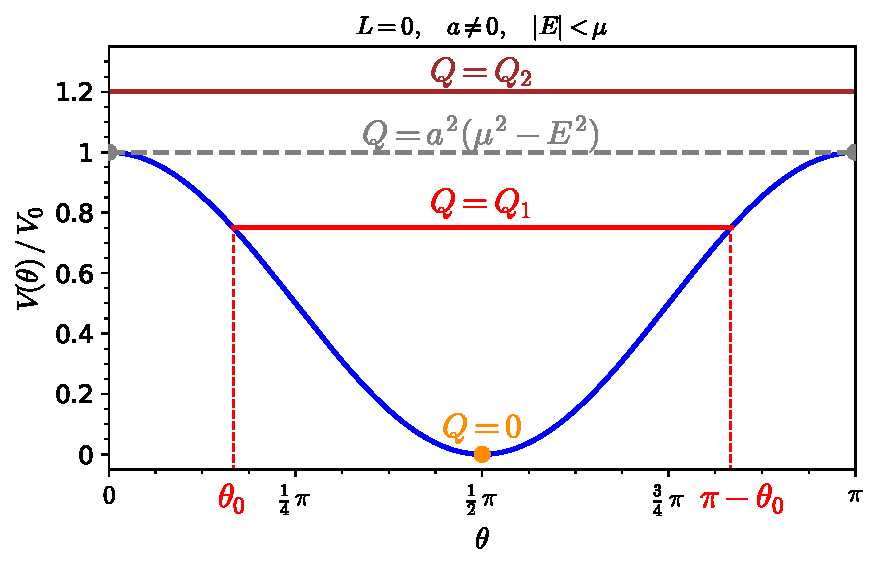
\includegraphics[height=0.24\textheight]{gek_th_pot_L_0_low_E.pdf}
\ 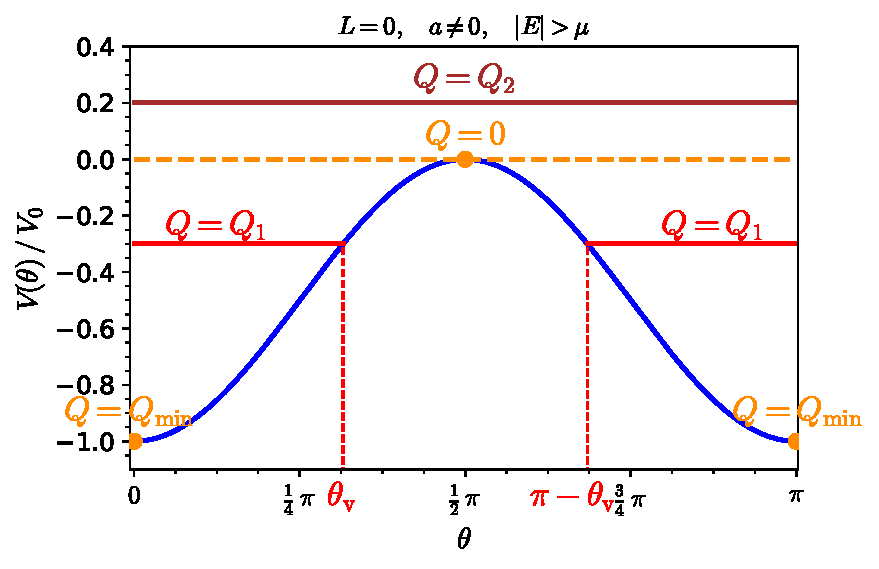
\includegraphics[height=0.24\textheight]{gek_th_pot_L_0_high_E.pdf}}
\caption[]{\label{f:gek:th_pot_L_0} \footnotesize
Effective $\th$-potential $V(\th)$ in the case $L=0$ and $a\neq 0$. $V(\th)$ is plotted
in units of $V_0 := a^2|\mu^2 - E^2|$.
The left figure is for $|E| < \mu$, with colored dots or horizontal lines
corresponding to geodesic trajectories for four values of the Carter constant $Q$:
$0$, $Q_1 = 0.75 V_0$, $a^2(\mu^2 - E^2)$ and $Q_2 = 1.2 V_0$.
The right figure is for $|E| > \mu$, with trajectories corresponding
to four values of $Q$: $Q_{\rm min} = -a^2(E^2 - \mu^2)$,
$Q_1 = -0.3 V_0$, $0$ and $Q_2 = 0.2 V_0$.
Dashed lines indicate trajectories with asympotic $\th$-values.
%\textsl{[Figure produced with the notebook \ref{s:sam:ges_eff_pot_null}]}
}
\end{figure}


\begin{figure}
\centerline{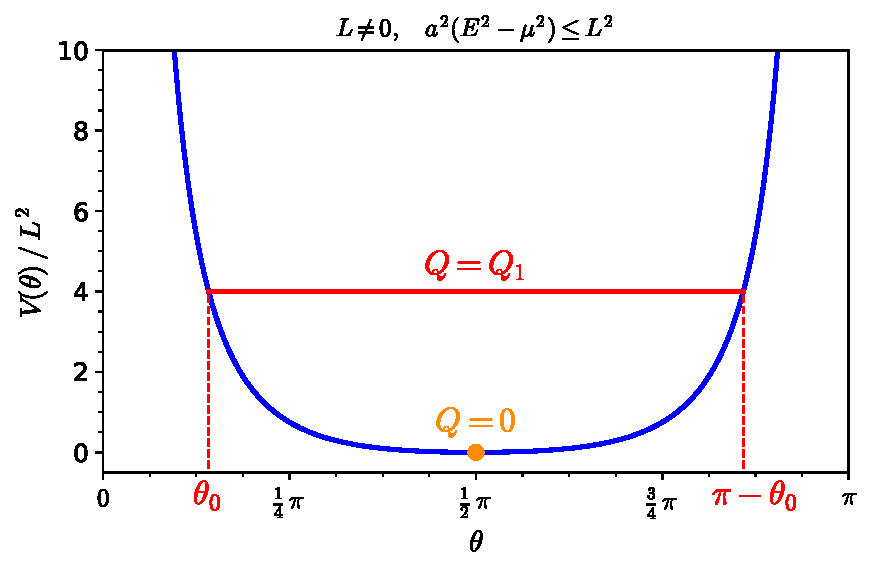
\includegraphics[width=0.49\textwidth]{gek_th_pot_high_L.pdf}
\ 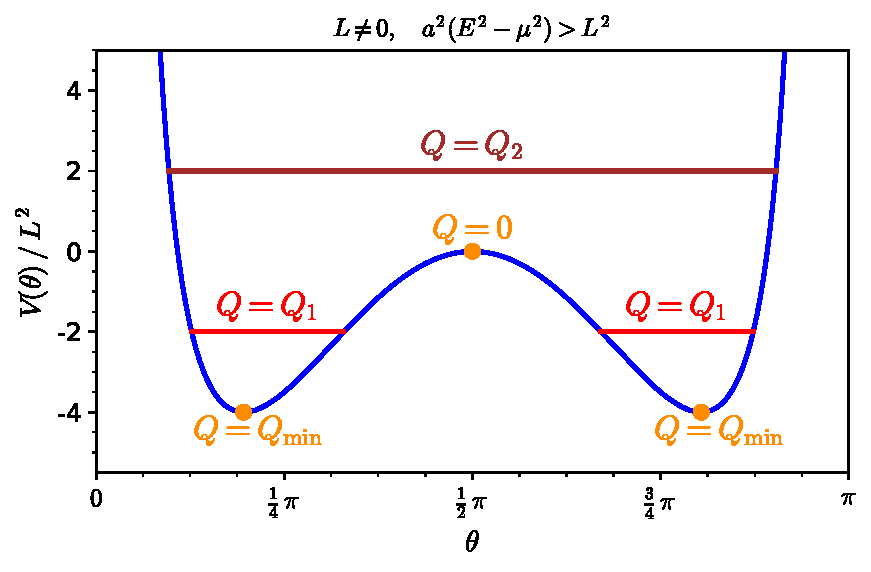
\includegraphics[width=0.49\textwidth]{gek_th_pot_low_L.pdf}}
\caption[]{\label{f:gek:th_pot_L_non0} \footnotesize
Effective $\th$-potential $V(\th)$ in the case $L\neq0$.
The left figure is for $a^2(E^2 - \mu^2) \leq L^2$, with
with colored dots or horizontal lines
corresponding to geodesic trajectories for
two values of the Carter constant $Q$: $0$ and $Q_1= 4 L^2$.
The right figure is for $a^2(E^2 - \mu^2) > L^2$, with trajectories corresponding
to four values of $Q$: $Q_{\rm min}$, $Q_1 = - 2 L^2$, $0$ and $Q_2 = 2 L^2$.
The dashed line ($Q=0$)
indicates the trajectory with an asympotic $\th$-value, which is $\pi/2$.
%\textsl{[Figure produced with the notebook \ref{s:sam:ges_eff_pot_null}]}
}
\end{figure}


\subsubsection{Geodesics with $L\not=0$}

When $L\not=0$, we see from expression~(\ref{e:gek:def_V_th}) that
$V(\th) \to +\infty$ when $\th\to 0$ or $\pi$.
We conclude immediately that the geodesic cannot reach the rotation axis
for $L\not=0$.
Moreover, we have
\[
    \derd{V}{\th} = - 2 \cos\th\sin\th \left[ a^2 (\mu^2 - E^2) + \frac{L^2}{\sin^4\th} \right] .
\]
The extrema of $V$ in $(0,\pi)$ are then given by
\be
    \derd{V}{\th} = 0 \iff
        \th = \frac{\pi}{2} \quad\mbox{or}\quad
        \sin^4\th = \frac{L^2}{a^2(E^2 - \mu^2)} .
\ee
We are thus led to distinguish two cases, depending whether or not the
equation involving $\sin^4\th$ has solutions distinct from $\pi/2$:
\begin{itemize}
\item \textbf{Case} $a^2(E^2 - \mu^2) \leq L^2 \iff a=0\
\mbox{or}\ |E| \leq \sqrt{\mu^2 + \frac{L^2}{a^2}}$: the only extremum solution is
$\th=\pi/2$.
Its value is $V(\pi/2)=0$ and it is
necessarily a miminum, since $V(\th) \to +\infty$ at the boundaries of the
interval $[0,\pi]$ (cf. left part of Fig.~\ref{f:gek:th_pot_L_non0}).
Hence one must have $Q\geq 0$, with
\begin{itemize}
\item $Q=0$: the geodesic stays stably in the
equatorial plane.
\item $Q>0$: the geodesic oscillates about the equatorial plane,
between two turning points at $\th=\th_0$ and $\pi-\th_0$, $\th_0$ being the solution
of $V(\th_0) = Q$ in $(0,\pi/2)$ (cf. the trajectory $Q=Q_1$ in Fig.~\ref{f:gek:th_pot_L_non0}, left).
\end{itemize}
\item \textbf{Case} $a^2(E^2 - \mu^2) > L^2 \iff a\neq 0\
\mbox{and}\ |E| > \sqrt{\mu^2 + \frac{L^2}{a^2}}$: $V(\th)$ has three extrema (cf. right part of Fig.~\ref{f:gek:th_pot_L_non0}), which are located at
$\th=\th_*$, $\pi/2$ and $\pi-\th_*$ with
\be
    \th_* := \arcsin\sqrt{\frac{|L|}{a\sqrt{E^2 - \mu^2}}}
    \quad\mbox{and}\quad 0 < \th_* < \frac{\pi}{2} .
\ee
$\th_*$ and $\pi-\th_*$ correspond to the minimum of $V(\th)$,
while $\pi/2$ corresponds to a local maximum. The minimum is
$V(\th_*) = (1-\sin^2\th_*)(a^2(\mu^2-E^2) + L^2/\sin^2\th_*) = - (a \sqrt{E^2 - \mu^2} - |L|)^2$.
This is necessary the minimal value of $Q$ [cf. Eq.~(\ref{e:gek:V_leq_Q})]:
\be
    Q_{\rm min} = - \left( a \sqrt{E^2 - \mu^2} - |L| \right) ^2 .
\ee
We have then (cf. right part of Fig.~\ref{f:gek:th_pot_L_non0})
\begin{itemize}
\item $Q = Q_{\rm min}$: the geodesic stays stably at a fixed value of $\th$,
either $\th_*$ or $\pi - \th_*$.
\item $Q_{\rm min} < Q < 0$: the geodesic oscillates between two turning
points either in the Northen
hemisphere ($\th < \pi/2$) or the Southern one ($\th > \pi/2$), without reaching
the equator nor the rotation axis (cf. the trajectories $Q=Q_1$ in Fig.~\ref{f:gek:th_pot_L_non0}, right).
\item $Q=0$: the geodesic lies unstably in the equatorial plane or
moves asymptotically towards it (possibly after a turning point at $\th_0\neq\pi/2$), $\pi/2$ being an asymptotic $\th$-value, since $\Theta'(\pi/2) = - V'(\pi/2)=0$
(cf. Sec.~\ref{s:gek:asymptotic_values}).
\item $Q>0$: the geodesic oscillates about the equatorial plane,
between two turning points at $\th=\th_0$ and $\pi-\th_0$, $\th_0$ being the solution
of $V(\th_0) = Q$ in $(0,\pi/2)$ (cf. the trajectory $Q=Q_2$ in Fig.~\ref{f:gek:th_pot_L_non0}, right).
\end{itemize}
\end{itemize}

We can summarize the above results by
\begin{greybox}
\begin{itemize}
\item A geodesic $\Li$ of Kerr spacetime cannot encounter the rotation axis unless it has $L=0$.
\item If $a=0$ (Schwarzschild limit) or $|E| \leq \sqrt{\mu^2 + \frac{L^2}{a^2}}$,
the Carter constant $Q$ is necessarily non-negative:
\be \label{e:gek:Q_nonnegative}
    Q \geq 0 .
\ee
\item The Carter constant $Q$ can take negative values if, and only if,
$a\neq 0$ and $|E| > \sqrt{\mu^2 + \frac{L^2}{a^2}}$; its range is then
limited from below:
\be
    Q \geq Q_{\rm min} = - \left( a \sqrt{E^2 - \mu^2} - |L| \right) ^2.
\ee
A geodesic with $Q<0$ is called \defin{vortical}\index{vortical geodesic}; it
never encounters the equatorial plane.
\item If $Q>0$, $\Li$ oscillates symmetrically about the equatorial plane,
between two turning points, $\th_0$ and $\pi-\th_0$, such that $0<\th_0<\pi/2$,
except for two subcases with $L=0$: (i) $Q = a^2 (\mu^2 - E^2)$: $\Li$
lies unstably along the rotation axis or approaches it asymptotically
and (ii) $Q >a^2(\mu^2 - E^2)$: $\Li$
crosses repeatedly the rotation axis, with $\th$ taking all values in the
range $[0,\pi]$.
\item If $Q=0$, $\Li$ is stably confined to the equatorial plane
for $a^2 (E^2 - \mu^2) < L^2$ or $a^2 (E^2 - \mu^2) = L^2 \neq 0$;
for $a^2 (E^2 - \mu^2) > L^2$, $\Li$ either lies unstably in the equatorial
plane or approaches it asymptotically from one side, while for $L=0$ and ($a=0$ or $|E|=\mu$),
$\Li$ lies at a constant value $\th=\th_0\in[0,\pi]$.
\item If $Q_{\rm min} < Q < 0$, $\Li$ oscillates between two turning
points strictly located in the Northern hemisphere ($0<\th<\pi/2$) or in
the Southern hemisphere ($\pi/2<\th<\pi$) for $L\neq 0$, while for $L=0$,
$\Li$ oscillates about the rotation axis, without encoutering the equatorial
plane, having a turning point at $\th_0$ such that $0<\th_0<\pi/2$
(motion in the Northern hemisphere) or $\pi/2<\th_0<\pi$
(motion in the Southern hemisphere).
\item If $Q = Q_{\rm min}$, $\Li$ lies stably at a constant value $\th=\th_0$,
with $\th_0 = 0$ or $\pi$ (the rotation axis) for $L=0$ and $0<\th_0< \pi/2$
or $\pi/2<\th_0<\pi$ for $L\neq 0$.
\end{itemize}
\end{greybox}

\begin{remark}
We could have deduced that $L=0$ is a necessary condition for a geodesic
to encounter the rotation axis without studying the potential $V(\th)$. Indeed,
by definition, $L = \w{\eta}\cdot\w{p}$ [Eq.~(\ref{e:gek:def_L})], with the Killing
vector $\w{\eta}$ being zero on the rotation axis, since the latter is
pointwise invariant under the action of the rotation group $\mathrm{SO}(2)$.
Hence $L=0$ on the rotation axis. Since $L$ is constant along the geodesic,
the result follows immediately.
\end{remark}

\begin{remark}
That a vortical geodesic never intersects the equatorial plane has been
obtained by examining the various cases $Q<0$. This result can be derived
directly from the constraint $\Theta(\th)\geq 0$ [Eq.~(\ref{e:gek:Theta_non_neg})],
by noticing the identity
$\Theta(\pi/2) = Q$, which follows immediately from Eq.~(\ref{e:gek:Theta_Q}).
\end{remark}

\begin{example}[Schwarzschild geodesics]
It is instructive to apply the above results to $a=0$ and recover
the geodesics in Schwarzschild spacetime studied in Chaps.~\ref{s:ges} and \ref{s:gis}.
There, spherical symmetry was used to select the coordinates $(t,r,\th,\ph)$ so that
the geodesic was confined to the hyperplane $\th=\pi/2$. Consequently there was
no $\th$-motion. Here, we keep the coordinates $(t,r,\th,\ph)$ fixed and do not
assume they are adapted to the geodesic $\Li$ under consideration. So $\th$
may vary along $\Li$. In Schwarzschild spacetime, the Carter constant $Q$
is always non-negative [Eq.~(\ref{e:gek:Q_nonnegative})].\\
If $Q=0$, then for $L=0$, $\Li$ lies at a constant value of $\th$: this actually
corresponds to a purely radial geodesic. Indeed,
the total angular momentum measured in the asymptotic region is $\w{L}_{\rm tot} = 0$
in that case [set $Q=0$, $L=0$ and $a=0$ in Eq.~(\ref{e:gek:Q_Ltot2_L2})].
If $L\neq 0$, still with $Q=0$,
$\Li$ lies stably in the equatorial plane (this is the only possibility for $a=0$ among
the $Q=0$ cases listed above).\\
If $Q>0$, then $L=0$ is necessarily the subcase (ii) listed above:
$\Li$ crosses repeatedly the $z$-axis ($\th\in\{0,\pi\}$); this corresponds to the case where
the orbital plane contains the $z$-axis. All the angular momentum measured asymptotically
is then contained in $Q$ [cf. Eq.~(\ref{e:gek:Q_Ltot2_L2})].
For $Q>0$ and $L\neq 0$, $\Li$ oscillates symmetrically about the equatorial
plane: this is the case where the orbital plane is inclined by an angle
$\iota\in(0,\pi/2)$
with respect to the equatorial plane; the $\th$-turning point of $\Li$ is then
$\th_0 = \pi/2-\iota$.
\end{example}


\subsection{$r$-motion}

Let us rewrite the first-order radial equation of motion (\ref{e:gek:drdl_Mino})
as
\be \label{e:gek:r_eff_potential}
   \encadre{ \left( \derd{r}{\lambda'} \right)^2 + U(r) = - a^2 Q },
\ee
where
\be \label{e:gek:U_R_Q}
    U(r) := - R(r) - a^2 Q .
\ee
$U(r)$ is a quartic polynomial, whose expression is obtained by expanding
Eq.~(\ref{e:gek:def_R}) in powers of $r$:
\be \label{e:gek:U_r_powers}
    \encadre{ U(r) = (\mu^2 - E^2) r^4 - 2 m \mu^2 r^3
     + \left[ Q + L^2 + a^2(\mu^2 - E^2) \right] r^2
     - 2m\left[ Q + (L - a E)^2 \right] r } .
\ee
As Eq.~(\ref{e:gek:th_eff_potential}) for $\th$, Eq.~(\ref{e:gek:r_eff_potential})
has the shape of the first integral of a 1-dimensional motion in the potential $U(r)$,
which we naturally call the \defin{effective $r$-potential}\index{effective!$r$-potential}.
Since $(\D r/\D \lambda')^2 \geq 0$, the motion is possible only when the
potential is lower than the ``total energy'' $-a^2 Q$:
\be \label{e:gek:U_leq_a2Q}
     U(r) \leq - a^2 Q .
\ee

\subsubsection{Geodesics with $|E|<\mu$}

For $r\to \pm\infty$ and $|E|\neq \mu$,
we have $U(r) \sim (\mu^2 - E^2) r^4$ and in
particular $\lim_{r\to\pm\infty} U(r) = - \infty$ for $|E|>\mu$
and $\lim_{r\to\pm\infty} U(r) = + \infty$ for $|E|<\mu$. In the latter case,
the constraint (\ref{e:gek:U_leq_a2Q}) cannot be satisfied for large values
of $|r|$. A geodesic with $|E|<\mu$ is therefore located within a bounded
region in terms of the radial coordinate $r$. Moreover, we have seen in
Sec.~\ref{s:gek:th_motion} that for $|E|<\mu$, one has $Q\geq 0$
[Eq.~(\ref{e:gek:Q_nonnegative})]. Therefore $-a^2 Q \leq 0$ and
(\ref{e:gek:U_leq_a2Q}) implies $U(r)\leq 0$. This cannot hold for $r<0$: we see
on expression~(\ref{e:gek:U_r_powers}) that for $|E|<\mu$ (which implies $\mu>0$ and $Q\geq 0$) and $r<0$, we have
\[
        U(r) = \underbrace{(\mu^2 - E^2) r^4}_{>0} \underbrace{- 2 m \mu^2 r^3}_{>0}
     + \underbrace{\left[ Q + L^2 + a^2(\mu^2 - E^2) \right] r^2}_{\geq 0}
     \underbrace{- 2m\left[ Q + (L - a E)^2 \right] r}_{\geq 0} > 0 .
\]
Hence we conclude:
\begin{greybox}
Any geodesic $\Li$ with $|E|<\mu$ is necessarily timelike ($\mu >0$),
has a non-negative Carter constant $Q$,
is confined to the region $r\geq 0$ of Kerr spacetime
and cannot reach arbitrary large values of $r$. $\Li$ is called a
\defin{geodesic with a bound orbit}\index{geodesic!with a bound orbit}\index{bound!orbit},
or in short, a \defin{bound geodesic}\index{bound!geodesic}.
\end{greybox}
\begin{remark} \label{r:gek:bound_geod}
That $\Li$
cannot reach the asymptotic region $r\to +\infty$ could have been
found directly from the definition of $E$ as the ``energy at infinity''
of the particle $\mathscr{P}$ having $\Li$ as worldline
[Eq.~(\ref{e:gek:def_E})]. Indeed, since $\Li$ is timelike, the 4-momentum
of $\mathscr{P}$ is $\w{p} = \mu \w{u}$ [Eq.~(\ref{e:fra:p_m_u})], where
$\w{u}$ is the 4-velocity of $\mathscr{P}$, so that Eq.~(\ref{e:gek:def_E})
yields $E = - \mu\, \w{\xi}\cdot\w{u}$. Now, when $r\to +\infty$, $\w{\xi}$
tends to the 4-velocity of a static inertial observer.
If $\Li$ could reach the asymptotic region,
the scalar
product of the two 4-velocities $\w{\xi}$ and
$\w{u}$ would be necessarily lower or equal to $-1$, or equivalently
$\Gamma := - \w{\xi}\cdot\w{u} \geq 1$ (the proof lies in expression
(\ref{e:fra:Gam_V2}) of $\Gamma$ with $0\leq \w{V}\cdot\w{V} < 1$), so that
we would have $E \geq \mu$, which contradicts $|E|<\mu$.
\end{remark}

\subsubsection{Geodesics with $|E|=\mu$}

Contrary to the case $|E|<\mu$, a geodesic with $|E|=\mu$ can be null,
provided it has $E=0$
(cf. Example~\ref{x:gek:null_generator_hor} on page~\pageref{x:gek:null_generator_hor}).
We have
\begin{greybox}
Any geodesic with $|E|=\mu$ has $Q\geq 0$ and is necessarily confined
to the region $r\geq 0$ of Kerr spacetime.
\end{greybox}
\begin{proof}
$Q\geq 0$ follows directly from the criteria $|E| \leq \sqrt{\mu^2 + {L^2}/{a^2}}$
[cf. Eq.~(\ref{e:gek:Q_nonnegative})],
which is evidently fulfilled for $|E|=\mu$.
Furthermore, for $|E|=\mu$, the expression of the effective $r$-potential simplifies to
\[
    U(r) = - 2 m \mu^2 r^3 + (Q + L^2) r^2 - 2m  \left[Q + (L-aE)^2 \right] r .
\]
For $r<0$, all the three terms in the above sum are $\geq 0$.
If $\Li$ is timelike, then $\mu>0$ and the first term is $>0$, so that
$r<0 \Rightarrow U(r) > 0$, which is incompatible with the constraint
(\ref{e:gek:U_leq_a2Q}) with $Q\geq 0$. Let us now assume that $\Li$ is null.
We have then $\mu=0$ and $E=0$, so that
\[
    U(r) = (Q + L^2) r^2 - 2m  (Q + L^2) r  = (Q+L^2) r ( r - 2m ) .
\]
If $Q + L^2 \neq 0$, $U(r)$ is a quadratic polynomial that is $>0$ outside
the interval $[0,2m]$. In particular, $U(r)>0$ for $r<0$. Once again, this contradicts
(\ref{e:gek:U_leq_a2Q}).
If $Q + L^2 = 0$, the property $Q\geq 0$ implies $Q=0$ and $L = 0$.
The Carter constant $\mathscr{K}$ is then zero as well, since
$\mathscr{K} = Q + (L - a E)^2$ [Eq.~(\ref{e:gek:def_Q})].
Then by the result (\ref{e:gek:all_const_zero}), $\Li$ is a null geodesic
generator of either the event horizon $\Hor$, which is located at $r=r_+$,
or the inner horizon $\Hor_{\rm in}$, which is located at $r=r_-$.
Since both $r_+$ and $r_-$ are positive
[Eq.~(\ref{e:ker:order_r_pm})], we cannot have $r<0$ in this case either.
\end{proof}

A timelike geodesic with $E=\mu$ can reach the asymptotic region
$r\to +\infty$. It has then a Lorentz factor
with respect to the asymptotic static observer of 4-velocity $\w{\xi}$
equal to one (cf. Remark~\ref{r:gek:bound_geod} above), which implies that
$\w{p}$ is collinear to $\w{\xi}$. In that sense, such a
geodesic is asymptotically ``at rest''.

On the opposite, a null geodesic with $E=\mu (=0)$
cannot reach the asymptotic region
$r\to +\infty$. Actually, it cannot even exist outside the ergoregion,
by virtue of the property (\ref{e:gek:E_positive}).
\begin{example}
The null geodesics generating the horizons $\Hor$ and $\Hor_{\rm in}$
considered in
Example~\ref{x:gek:null_generator_hor} on page~\pageref{x:gek:null_generator_hor}
have $E=0$ [Eq.~(\ref{e:gek:generator_hor_E_L_zero})]
and are indeed fully located inside the ergoregion $\mathscr{G}$,
since $\Hor\subset\mathscr{G}$ and $\Hor_{\rm in}\subset\mathscr{G}$
(cf. Fig.~\ref{f:ker:ergo_a90}).
\end{example}

\subsubsection{Geodesics with $|E|>\mu$}

An immediate corollary of the properties obtained for $|E|<\mu$ and $|E|=\mu$
is
\begin{greybox}
Only geodesics with $|E| > \mu$ can have some part in the region $r<0$ of Kerr spacetime, $\M_-$:
\be
    \Li \cap \M_- \neq \varnothing \Longrightarrow |E| > \mu .
\ee
\end{greybox}

\subsection{Geodesics reaching or emanating from the ring singularity}

In the Schwarzschild spacetime, any causal geodesic that enters into the black
hole region inevitably terminates at the curvature singularity $r=0$, as it
is clear on the Kruskal or Carter-Penrose diagrams constructed in Chap.~\ref{s:max}.
For the Kerr spacetime with $a\neq 0$, we are going to see that, on the contrary,
most causal geodesics in the black hole region \emph{avoid} the curvature
singularity. In all this section, we assume $a\neq 0$, so that the
curvature singularity is the ring singularity\index{ring!singularity} $\ring$
discussed in Sec.~\ref{s:ker:singularities}.

Formally, $\ring$ is not
part of the Kerr spacetime $\M$ but of the larger manifold $\R^2\times\mathbb{S}^2$
[cf. the construction (\ref{e:ker:def_M_Kerr_spacetime})]. It is located
at located at $\rho^2 = 0$, i.e. at $r=0$ and
$\th=\pi/2$. We shall say that a
geodesic $\Li$ of affine parameter $\lambda$ (oriented towards to the future)
\defin{approaches the ring singularity}\index{approach the singularity}
if $\Li$ has both
$r(\lambda)\to 0$ and $\th(\lambda) \to 0$ as $\lambda\to\lambda_*$, with
$\lambda_*$ finite or infinite. If $\lambda_*$ is finite, we shall say
that $\Li$ \defin{hits the ring singulary}\index{hit the singularity}
for $\lambda\to\lambda_*^-$ and
\defin{emanates from the ring singularity}\index{emanate from the singularity}
for $\lambda\to\lambda_*^+$. If $\lambda_*=\pm\infty$, we shall say
that $\Li$ \defin{asymptotically approaches the ring singularity}\index{asymptotically!
approach the singularity}.

A first key result is
\begin{greybox}
A null or timelike geodesic $\Li$ that approaches the ring singularity has
a vanishing Carter constant $Q$.
\end{greybox}
\begin{proof}
From Eqs.~(\ref{e:gek:def_R}) and (\ref{e:gek:Theta_Q}), we have
\[
 \lim_{r\to 0} R(r) = - a^2 Q \quad\mbox{and}\quad
 \lim_{\th\to \pi/2} \Theta(\th) = Q .
\]
The constraints $R(r) \geq 0$ [Eq.~(\ref{e:gek:R_non_neg})]
and $\Theta(\th)\geq 0$ [Eq.~(\ref{e:gek:Theta_non_neg})] imply then respectively
$Q \leq 0$ and $Q\geq 0$, from which we get $Q=0$.
\end{proof}

The above property can be refined\footnote{This is a refinement because not all
geodesics with $Q=0$ lie in the equatorial plane. For instance the
null geodesic generators of the event horizon $\Hor$ have $Q=0$ [Eq.~(\ref{e:gek:all_const_zero})]
but those with $\th\neq \pi/2$ lie outside the equatorial plane.}:
\begin{greybox}
A null or timelike geodesic cannot approach the ring singularity unless it lies
entirely in the equatorial plane.
\end{greybox}
\begin{proof}
Let $\Li$ be a causal geodesic that approaches $\ring$. From the previous result,
$\Li$ has $Q=0$. Reviewing the subcases $Q=0$ among all the cases considered in
Sec.~\ref{s:gek:th_motion}, we see that $\Li$ can approach $\th=\pi/2$ iff
(i) $\Li$ has
$|E|\leq \sqrt{\mu^2 + L^2/a^2}$ and lies stably in the equatorial plane
or (ii) $\Li$ has $|E| > \sqrt{\mu^2 + L^2/a^2}$ and approaches asymptotically
$\th=\pi/2$ as the Mino time $\lambda'\to \pm\infty$.
Let us show that (ii) is not compatible with $r\to 0$.
For $Q=0$, we have [cf. Eqs.~(\ref{e:gek:U_R_Q}) and (\ref{e:gek:U_r_powers})]:
\[
 R(r) = r \left[ (E^2 - \mu^2) r^3 + 2 m \mu^2 r^2
     + \left( a^2(E^2 - \mu^2) - L^2 \right) r
     + 2m (L - a E)^2 \right] ,
\]
with the constant term inside the square brackets $2m(L - a E)^2 \neq 0$,
since $L=a E$ is not compatible with $|E| > \sqrt{\mu^2 + L^2/a^2}$. It
follows that $r=0$ is a simple root of $R(r)$. If $\Li$ reaches both
$r=0$ and $\th=\pi/2$ when $\lambda\to\lambda_*$, from some point $(r_0,\th_0)$,
then we should have, by virtue of
Eqs.~(\ref{e:gek:Minotime_r_slash_int}) and (\ref{e:gek:Minotime_th_slash_int}),
\be \label{e:gek:dashint_r_theta}
    \lambda'_* - \lambda'_0 = \dashint_{r_0}^0 \frac{\eps_r \, \D r}{\sqrt{R(r)}}
    = \dashint_{\th_0}^{\frac{\pi}{2}} \frac{\eps_\th \, \D \th}{\sqrt{\Theta(\th)}} ,
\ee
where $\lambda'_*$ is the Mino time corresponding to $\lambda_*$. Note that
$\lambda'_*$ may be infinite even if $\lambda_*$ is finite, due to the
relation (\ref{e:gek:def_Mino_time}) with $\rho^2\to 0$ when $\lambda\to\lambda_*$.
Since $r=0$ is a simple root of $R(r)$, the integral on $r$ has a finite value.
Now, for $Q=0$, expression (\ref{e:gek:Theta_Q}) for $\Theta$ reduces to
\[
    \Theta(\th) = \cos^2\th \left[ a^2 (E^2 - \mu^2)
    - \frac{L^2}{\sin^2\th} \right] .
\]
The $\cos^2\th$ term, which behaves as $(\th - \pi/2)^2$ near $\pi/2$,
makes the ingetral on $\th$ in
Eq.~(\ref{e:gek:dashint_r_theta}) divergent, which is incompatible with the
finite value of the integral on $r$ in the left-hand side. Hence only (i) is possible, which completes
the proof.
\end{proof}

The above result has been obtained for a generic approach to the ring singularity,
i.e. for a geodesic $\Li$ that hits $\ring$, emanates from $\ring$ or
asymptotically approach $\Li$ in the future or the past. If we apply it to
null geodesics (light rays) emanating from $\ring$, we conclude that an intrepid observer
diving into the black hole would not see the ring singularity at all, except when
he crosses the equatorial plane. At this instant, the singularity would appear
to him as a 1-dimensional segment, and the image would disappear as soon as the observer
leaves the equatorial plane. In particular, the observer will never see a ring-like image.


%\subsection{Moving to the negative $r$ side}


\section{Timelike geodesics}

\subsection{Parametrization}

\subsection{Bound geodesics}

\subsection{Equatorial geodesics}

%%%%%%%%%%%%%%%%%%%%%%%%%%%%%%%%%%%%%%%%%%%%%%%%%%%%%%%%%%%%%%%%%%%%%%%%%%%%%%%

\section{Null geodesics}

\subsection{Parametrization}

\subsection{Principal null geodesics}

\subsection{Spherical null geodesics}






Circular orbits in Kerr spacetime: \cite{BardePT72} (see also \cite{Barde73})

More general orbits: \cite{Perez-Giz11}, \cite{GrossLP12}
